\documentclass[11pt]{article}

% Required packages for formatting
\usepackage[margin=1in]{geometry}      % 1-inch margins on all sides
\usepackage{setspace}                   % Control line spacing
\usepackage{amsmath}                    % Mathematics
\usepackage{amssymb}                    % Mathematical symbols
\usepackage{amsthm}                     % Theorem environments
\usepackage[ruled,vlined,linesnumbered]{algorithm2e} % Pseudocode
\usepackage{tikz}                       % Drawings
\usepackage{graphicx}                   % Graphics inclusion
\usepackage{cite}                       % Citation formatting
\usepackage{float}
\usepackage{hyperref}                   % Hyperlinks
\SetArgSty{textnormal}


% temporary for comments:
\newcommand{\DD}[1]{\textcolor{red}{DD: #1}}
\newcommand{\DDfix}[1]{\textcolor{violet}{#1}}

% Define colors
\definecolor{cutA}{RGB}{214,39,40}
\definecolor{cutB}{RGB}{31,119,180}
\definecolor{cutC}{RGB}{44,160,44}
\definecolor{cutD}{RGB}{23,190,207}
\definecolor{cutE}{RGB}{148,103,189}
\definecolor{cutF}{RGB}{140,86,75}

% Bracket and notation macros
\newcommand{\br}[1]{\mathopen{}\left( #1 \right)}
\newcommand{\brc}[1]{\mathopen{}\left\{ #1 \right\}}
\newcommand{\spr}[1]{\mathopen{}\left| #1 \right|}
\newcommand{\fl}[1]{\mathopen{}\left\lfloor #1 \right\rfloor}
\newcommand{\cl}[1]{\mathopen{}\left\lceil #1 \right\rceil}
\newcommand{\angl}[1]{\mathopen{}\langle #1 \rangle}
\newcommand{\e}[1]{\exp\left\{ #1 \right\}}

% Algorithm and notation
\newcommand{\Cent}{\texttt{Cent}}
\newcommand{\APP}{\texttt{APP}}
\newcommand{\OPT}{\texttt{OPT}}
\newcommand{\COST}{{c}}
\newcommand{\dist}{\text{dist}}

% Calligraphic letter macros
\newcommand{\cA}{\mathcal{A}}
\newcommand{\cB}{\mathcal{B}}
\newcommand{\cC}{\mathcal{C}}
\newcommand{\cD}{\mathcal{D}}
\newcommand{\cE}{\mathcal{E}}
\newcommand{\cF}{\mathcal{F}}
\newcommand{\cG}{\mathcal{G}}
\newcommand{\cH}{\mathcal{H}}
\newcommand{\cI}{\mathcal{I}}
\newcommand{\cJ}{\mathcal{J}}
\newcommand{\cK}{\mathcal{K}}
\newcommand{\cL}{\mathcal{L}}
\newcommand{\cM}{\mathcal{M}}
\newcommand{\cN}{\mathcal{N}}
\newcommand{\cO}{\mathcal{O}}
\newcommand{\cP}{\mathcal{P}}
\newcommand{\cQ}{\mathcal{Q}}
\newcommand{\cR}{\mathcal{R}}
\newcommand{\cS}{\mathcal{S}}
\newcommand{\cT}{\mathcal{T}}
\newcommand{\cU}{\mathcal{U}}
\newcommand{\cV}{\mathcal{V}}
\newcommand{\cW}{\mathcal{W}}
\newcommand{\cX}{\mathcal{X}}
\newcommand{\cY}{\mathcal{Y}}
\newcommand{\cZ}{\mathcal{Z}}


\newtheorem{theorem}{Theorem}[section]
\newtheorem{lemma}[theorem]{Lemma}
\newtheorem{corollary}[theorem]{Corollary}
\theoremstyle{definition}
\newtheorem{observation}[theorem]{Observation}




% Formatting
\singlespacing                          % Single spacing between lines
\setlength{\parindent}{0.5in}          % Paragraph indentation
\setlength{\parskip}{12pt}             % Ample spacing between paragraphs

% Title, author, date
\title{Hierarchical $\cF$-Clustering: Approximation and Hardness of Clustering into Trees and Bounded Diameter Graphs}
\author{Anonymous Authors}
\date{}

\begin{document}

% Title page
\maketitle

% Abstract
\begin{abstract}
    Consider the following variation on the classical \textsc{Hierarchical Clustering} problem: Usually, while building a hierarchical clustering, one recursively partitions the data until each cluster becomes a singleton. In our setup, we relax the halting condition of the recursive process to stop whenever the remaining cluster is a graph belonging to a given class $\mathcal{F}$. We call this problem \textsc{Hierarchical $\mathcal{F}$-Clustering} and we measure the quality of any solution using adapted Dasgupta's clustering objective. We study two natural choices of $\mathcal{F}$: trees, denoted by $\mathcal{T}$ and graphs of diameter bounded by~$d$, denoted by $\mathcal{D}_d$ (which includes cliques for $d=1$).

    Hereby, we present the first polynomial time $\mathcal{O}(\log n\cdot\log\log n)$ and $\mathcal{O}(\log n)$-approximation algorithms for clustering into $\mathcal{T}$- and $\mathcal{D}_d$-clusters respectively.
    Our main technical contribution is a framework for approximating such problems based on linear programming. In fact, we characterize graphs classes $\mathcal{F}$ for which our approach can be applied and show that it includes both trees and bounded diameter graphs. However, our ideas are not limited to them and might be useful for other structures as well. Broadly speaking, our framework applies whenever the corresponding flat clustering problem, which we call \textsc{$p_{\mathcal{F}}$-Partitioning}, admits a natural ILP formulation together with a rounding procedure with provable approximation guarantees. Intuitively, given a set of vertices called terminals, the problem is to find an edge set whose removal results in satisfying certain vertex-dependent structural predicate for each terminal. For example, excluding all cycles going through terminals or ensuring that the diameter of all clusters with respect to the terminals is not too large. We then use these ingredients to build clustering trees with the aforementioned approximation guarantees. To complement these results, we show that both \textsc{Hierarchical $\mathcal{T}$-Clustering} and \textsc{Hierarchical $\mathcal{D}_d$-Clustering} cannot be approximated within any constant factor under the \textsc{Small Set Expansion Hypothesis}.
\end{abstract}


% Keywords
\noindent
\textbf{Keywords:} Hierarchical $\cF$-Clustering, Feedback Edge Set, Min-Multicut, $\rho$-Separator, Approximation Algorithms, Linear Programming.

\bigskip

\section{Introduction}
Hierarchical clustering is a way to recursively partition a dataset into clusters. The data is usually represented by a weighted, connected graph $G = (V, E, c)$, where $c\colon E\to \mathbb{N}$ is the \emph{similarity} measure between the points. The goal is to find a rooted tree called \textit{clustering tree} $T$, in which every node $u\in V\br{T}$ represents a connected component $G_u\subseteq G$ called a \textit{cluster}. Moreover, every non-leaf node $u$ of $T$ corresponds to a subset of edges $S_u$ such that for every child node $v$ of $u$, $G_v\in G_u\setminus S_u$. For each leaf node $l\in V\br{T}$ it is required that $G_l$ is a singleton, i.~e., $\spr{V\br{G_l}}=1$. Then, the \textit{Dasgupta's clustering objective} is defined as $\COST_G\br{T} = \sum_{u\in V\br{T}} c(S_u) \cdot |V(G_u)|$\footnote{Note that the usual way of defining the Dasgupta's clustering objective is $\COST_G\br{T} = \sum_{uv\in E} c(uv) \cdot |\ell_T\br{u,v}|$, where $\ell_T\br{u,v}$ denotes the smallest subtree containing both $u$ and $v$. It is easy to see, that our formulation is equivalent and we use it for the sake of convenience.}. The problem of finding a clustering tree which minimizes the above cost is known as the \textsc{Hierarchical Clustering} problem and is NP-hard~\cite{ACostFunctionForSimilarityBasedHierarchicalClustering}. Intuitively, the Dasgupta's clustering objective `punishes' cutting edges with high similarity early on in the clustering tree, since the larger the component in which the edge is cut, the higher the contribution of this edge to the cost.

The main advantage of the hierarchical clustering over various kinds of flat clustering is that it provides a decomposition of the data which is not reliant on the granularity of subdivision one wishes to acquire. Since the clusters are refined until they become singletons, the hierarchy encodes various granularity levels into it. However, it is often implicitly assumed that eventually all of them need to become singletons. In this work we ask the following question: What would happen if we relax the halting condition of the recursive partitioning process and allow it to stop whenever the remaining cluster is a graph of some class $\cF$? 
We will assume, that the graph class $\cF$ is a part of the input and represents some kind of structural property which is deemed `simple' enough so that there is no need to further refine the clusters\footnote{Here, we assume that $\cF$ is non-empty and closed under taking subgraphs, which ensures that any subcluster of a cluster in $\cF$ also belongs to $\cF$. Moreover, for the sake of practicality it is reasonable to assume that the class $\cF$ is recognizable in polynomial time. Otherwise, the task of constructing any clustering tree at all becomes intractable and the pursuit of approximation algorithms becomes futile as well.}.
Therefore we only require that for each leaf node $l\in V\br{T}$, $G_l\in \cF$. We call this problem \textsc{Hierarchical $\cF$-Clustering} (HC-$\cF$). The goal is again to minimize $\COST_G\br{T} = \sum_{u\in V\br{T}} c(S_u) \cdot |V(G_u)|$. For a visual example of a clustering tree for \textsc{HC-$\cT$}, where $\cT$ denotes the class of trees see Figure~\ref{fig:hac-intro-example}.
\DDfix{
We note that the objective value for HC-$\cF$ may be quite different from that of the classical hierarchical clustering.
If the input graph $G$ belongs to $\cF$, then $\COST_G\br{T}=0$ for a single-node $T$ with root representing $G$.
On the other hand, one may have, even for unit costs, $\COST_G\br{T}=\Omega\br{n^2}$ for $T$ whose leaves are singletons.
}
\begin{figure}[H]
    \centering
    \begin{minipage}[t]{0.46\textwidth}
        \centering
        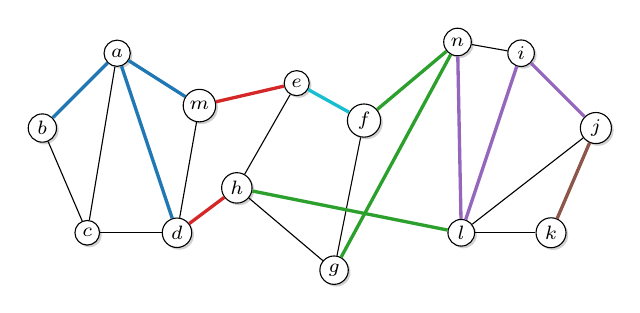
\begin{tikzpicture}[scale=0.95, every node/.style={circle,draw,fill=white,inner sep=1.5pt,font=\scriptsize,preaction={fill=black,opacity=0.18,transform canvas={xshift=0.8pt,yshift=-0.8pt}}}]
            \node (a1) at (-2.6,1.8) {$a$};
            \node (a2) at (-3.6,0.8) {$b$};
            \node (a3) at (-3.0,-0.6) {$c$};
            \node (a4) at (-1.8,-0.6) {$d$};
            \draw[cutB,very thick] (a1)--(a2);
            \draw (a2)--(a3);
            \draw (a3)--(a4);
            \draw[cutB,very thick] (a4)--(a1);
            \draw (a1)--(a3);

            \node (b1) at (-0.2,1.4) {$e$};
            \node (b2) at (0.7,0.9) {$f$};
            \node (b3) at (0.3,-1.1) {$g$};
            \node (b4) at (-1.0,0.0) {$h$};
            \draw[cutD,very thick] (b1)--(b2);
            \draw (b2)--(b3);
            \draw (b3)--(b4);
            \draw (b4)--(b1);

            \node (c1) at (2.8,1.8) {$i$};
            \node (c2) at (3.8,0.8) {$j$};
            \node (c3) at (3.2,-0.6) {$k$};
            \node (c4) at (2.0,-0.6) {$l$};
            \draw[cutE,very thick] (c1)--(c2);
            \draw[cutF,very thick] (c2)--(c3);
            \draw (c3)--(c4);
            \draw[cutE,very thick] (c4)--(c1);
            \draw (c2)--(c4);

            \node (x1) at (-1.5,1.1) {$m$};
            \node (x2) at (1.95,1.95) {$n$};
            \draw[cutB,very thick] (x1)--(a1);
            \draw (x1)--(a4);
            \draw[cutA,very thick] (x1)--(b1);
            \draw[cutC,very thick] (x2)--(b2);
            \draw[cutC,very thick] (x2)--(b3);
            \draw (x2)--(c1);
            \draw[cutE,very thick] (x2)--(c4);
            \draw[cutA,very thick] (a4)--(b4);
            \draw[cutC,very thick] (b4)--(c4);
        \end{tikzpicture}
        \\\smallskip
        {\small An input graph $G$ with 14 vertices.
        For all edges $e$, we have $c(e)=1$.}
    \end{minipage}
    \begin{minipage}[t]{0.52\textwidth}
        \centering
        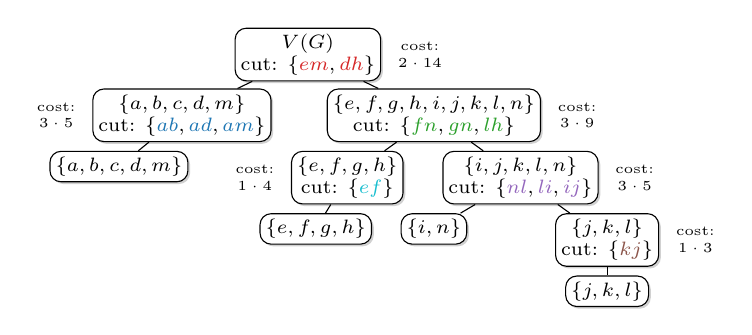
\begin{tikzpicture}[x=0.85cm,y=0.72cm, hcnode/.style={draw,rounded corners,fill=white,inner sep=2pt,font=\scriptsize,align=center,preaction={fill=black,opacity=0.18,transform canvas={xshift=0.8pt,yshift=-0.8pt}}}]
            \node[hcnode] (r) at (0,0) {$V(G)$\\cut: $\{\textcolor{cutA}{em},\textcolor{cutA}{dh}\}$};
            \node[hcnode,anchor=north] (u1) at ([xshift=-1.60cm,yshift=-0.09cm]r.south) {$\{a,b,c,d,m\}$\\cut: $\{\textcolor{cutB}{ab},\textcolor{cutB}{ad},\textcolor{cutB}{am}\}$};
            \node[hcnode,anchor=north] (u2) at ([xshift=1.60cm,yshift=-0.09cm]r.south) {$\{e,f,g,h,i,j,k,l,n\}$\\cut: $\{\textcolor{cutC}{fn},\textcolor{cutC}{gn},\textcolor{cutC}{lh}\}$};
            \node[hcnode,anchor=north] (v1) at ([xshift=-0.80cm,yshift=-0.11cm]u1.south) {$\{a,b,c,d,m\}$};
            \node[hcnode,anchor=north] (w1) at ([xshift=-1.10cm,yshift=-0.11cm]u2.south) {$\{e,f,g,h\}$\\cut: $\{\textcolor{cutD}{ef}\}$};
            \node[hcnode,anchor=north] (w2) at ([xshift=1.10cm,yshift=-0.11cm]u2.south) {$\{i,j,k,l,n\}$\\cut: $\{\textcolor{cutE}{nl},\textcolor{cutE}{li},\textcolor{cutE}{ij}\}$};
            \node[hcnode,anchor=north] (z1) at ([xshift=-0.40cm,yshift=-0.11cm]w1.south) {$\{e,f,g,h\}$};
            \node[hcnode,anchor=north] (z2) at ([xshift=-1.10cm,yshift=-0.11cm]w2.south) {$\{i,n\}$};
            \node[hcnode,anchor=north] (z3) at ([xshift=1.10cm,yshift=-0.11cm]w2.south) {$\{j,k,l\}$\\cut: $\{\textcolor{cutF}{kj}\}$};
            \node[hcnode,anchor=north] (t1) at ([xshift=0.00cm,yshift=-0.11cm]z3.south) {$\{j,k,l\}$};

            \node[draw=none,fill=none,preaction={},anchor=west,xshift=0.09cm,font=\tiny,align=center] at (r.east) {cost:\\$2\cdot 14$};
            \node[draw=none,fill=none,preaction={},anchor=east,xshift=-0.09cm,font=\tiny,align=center] at (u1.west) {cost:\\$3\cdot 5$};
            \node[draw=none,fill=none,preaction={},anchor=west,xshift=0.09cm,font=\tiny,align=center] at (u2.east) {cost:\\$3\cdot 9$};
            \node[draw=none,fill=none,preaction={},anchor=east,xshift=-0.09cm,font=\tiny,align=center] at (w1.west) {cost:\\$1\cdot 4$};
            \node[draw=none,fill=none,preaction={},anchor=west,xshift=0.09cm,font=\tiny,align=center] at (w2.east) {cost:\\$3\cdot 5$};
            \node[draw=none,fill=none,preaction={},anchor=west,xshift=0.09cm,font=\tiny,align=center] at (z3.east) {cost:\\$1\cdot 3$};

            \draw (r)--(u1);
            \draw (r)--(u2);
            \draw (u1)--(v1);
            \draw (u2)--(w1);
            \draw (u2)--(w2);
            \draw (w1)--(z1);
            \draw (w2)--(z2);
            \draw (w2)--(z3);
            \draw (z3)--(t1);
        \end{tikzpicture}
        \\\smallskip
        {\small A hierarchical clustering tree $T$ of cost $2\cdot14+3\cdot5+3\cdot9+1\cdot4+3\cdot5+1\cdot3=92$.}
    \end{minipage}
    \caption{Example of an instance of \textsc{HC-$\cT$} and a feasible hierarchical clustering: Colors denote edges cut at different levels of the tree.}
    \label{fig:hac-intro-example}
\end{figure}


\subsection{Motivations and applications}
Hierarchical clustering is a clustering technique that is far richer in structure and applications than traditional flat clustering. Since such an object encodes a hierarchical decomposition of data, one may choose an appropriate granularity level of clustering according to their needs. 
Phylogenetic trees, file systems, company management hierarchies, and socio-political divisions are all examples of hierarchical clusterings. Relaxing the halting condition of the clustering process has intuitive applications both for the case of trees as well as bounded-diameter graphs. It is easy to see, that not all of the aforementioned hierarchies finish on singleton objects. For example file systems often contain directories with multiple files. To seek more such examples, one may consider a categorization of products available in a given online store, where one bottom category may contain a very large amount of objects. It seems desirable to find a way to systematically build such structures, especially since a well-structured e-commerce platform is crucial for the success of the business. Here, it would be required for the bottom clusters to consists of products which are similar enough to be considered as a single category.
Enforcing bounded-diameter clusters is therefore a natural requirement, since such clusters aggregate points that are close to one another. Note, that in our setting, the cost function encodes similarity between objects, which inflates the diameter of the clusters when the similarity is higher. Luckily, it turns out that our diameter restrictions can be defined with respect to any metric, not limited to the similarity function or the number of edges.
% Trees are among simplest classes of graphs and therefore most of their structural properties are well understood. Additionally, many problems which are hard on general graphs can be solved efficiently on trees.  

Among possible usages of clustering into trees is the following heuristic for the standard \textsc{HC}. Firstly, run an algorithm for \textsc{HC-$\cT$} to obtain a clustering tree $T$ such that for each leaf $l$ of $T$, $G_l$ is a tree. Next, for each such $G_l$, run any algorithm for \textsc{HC} on trees to recover the remaining levels of clusterization. Since \textsc{HC} on trees admits a polynomial-time constant-factor approximation~\cite{ApproximateHierarchicalClusteringViaSparsestCutAndSpreadingMetrics}, the dominant part of the total approximation error comes from computing the solution for \textsc{HC-$\cT$}. Consequently, the better the approximation algorithm for \textsc{HC-$\cT$}, the better the performance of this heuristic.
The resulting clustering tree can also be used partially dynamically: the $\cT$-clustering tree may be stored statically, and whenever a leaf cluster needs refinement, we can run an \textsc{HC} algorithm on that leaf. In this way, we obtain a partially dynamic clustering tree which occupies less space than a full \textsc{HC} tree, while still allowing on-demand refinement.


% \begin{figure}[H]
    \centering
    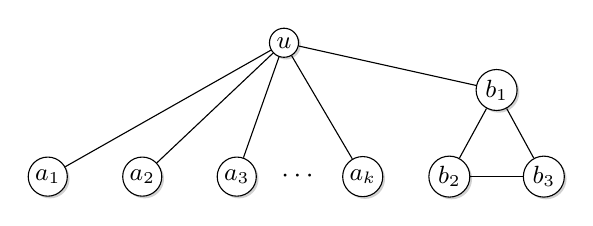
\begin{tikzpicture}[vtx/.style={circle,draw,fill=white,inner sep=1.4pt,font=\small,preaction={fill=black,opacity=0.18,transform canvas={xshift=0.8pt,yshift=-0.8pt}}}]
        \node[vtx] (u) at (0.8,0) {$u$};
        \node[vtx] (a1) at (-2.2,-1.7) {$a_1$};
        \node[vtx] (a2) at (-1.0,-1.7) {$a_2$};
        \node[vtx] (a3) at (0.2,-1.7) {$a_3$};
        \node[vtx] (ak) at (1.8,-1.7) {$a_k$};
        \node (dots) [draw=none,fill=none,preaction={},shape=rectangle,inner sep=0pt,outer sep=0pt,minimum size=0pt] at (1.0,-1.7) {$\cdots$};

        \node[vtx] (b1) at (3.5,-0.6) {$b_1$};
        \node[vtx] (b2) at (2.9,-1.7) {$b_2$};
        \node[vtx] (b3) at (4.1,-1.7) {$b_3$};

        \draw (u) -- (a1);
        \draw (u) -- (a2);
        \draw (u) -- (a3);
        \draw (u) -- (ak);
        \draw (u) -- (b1);

        \draw (b1) -- (b2);
        \draw (b2) -- (b3);
        \draw (b3) -- (b1);
    \end{tikzpicture}
    \caption{Example of graph for which the multiplicative difference between values of both clustering objective functions is $\Theta\br{n}$.}
    \label{fig:star-triangle-example}
\end{figure}

%
% We also remark that despite their similarity, the objective value of \textsc{HC-$\cF$} can be much smaller than that of \textsc{HC}. Consider $\cF=\cT$. Let $G$ be a star in which one vertex is replaced by a triangle, and assume uniform edge costs. The optimal clustering tree for \textsc{HC} has cost $\Omega\br{n^2}$, since at least $(n-2)/2$ vertices must have at least $(n-2)/2$ edges cut before becoming singletons. In contrast, the optimal clustering tree for \textsc{HC-$\cT$} has cost $n$, since the optimum consists of cutting a single edge of the triangle. This example shows that the structure of the optimum clustering tree for \textsc{HC-$\cT$} can differ significantly from \textsc{HC}. A similar example for $_d$-clusters is obtained by picking $d=1$ and letting the input graph be a clique. Here, the optimal clustering tree for \textsc{HC} has cost $\Omega\br{n^2}$, while the optimal clustering tree for \textsc{HC-$\cD_1$} has cost $0$, since the whole graph is a valid cluster.

\subsection{Our results and techniques}

Our main contribution is a general framework for approximating \textsc{HC-$\cF$} problems for classes of graphs $\cF$, which we call $\alpha\br{n}$-well-behaved. This means, that there exists a natural, cover-like ILP formulation of the \textsc{$p_{\cF}$-Partitioning} (\textsc{$p_{\cF}$-P}) problem (see Problem~\ref{prob:pfp}) as well as an algorithm which given a solution to the LP relaxation of this ILP, finds a solution to \textsc{$p_{\cF}$-P} with cost at most $\alpha\br{n}$ times the cost of the LP solution. This results in an $O\br{\alpha\br{n}+\beta\br{n}}$-approximation algorithm for \textsc{HC-$\cF$}, where $\beta\br{n}$ is the approximation ratio of the LP-based bicriteria algorithm for \textsc{$\rho$-SEP} (Problem~\ref{prob:rho-sep}), currently at $\beta\br{n}=O\br{\log n}$. As an immediate corollary we obtain an $O\br{\log n\cdot\log\log n}$-approximation algorithm for clustering into trees and an $O\br{\log n}$-approximation algorithm for clustering into clusters of diameter at most $d$. To the best of our knowledge, these are the first algorithmic results for the \textsc{HC-$\cF$} problem.

Conceptually, our work follows an implicitly, but broadly used technique which hereby we call \textit{flattening}. The idea is to subdivide the problem of finding a hierarchical/temporal\footnote{It is worth mentioning, that the hierarchical clustering tree can be treated as a sort of schedule of edges to be cut. This interpretation suggest that the depth of the tree can be treated as the time dimension of that schedule.} object such as a clustering tree into a problem of finding a sequence of `flat' objects such as separators or cuts. Among multiple uses of such a technique, one can mention \textsc{Hierarchical Clustering}~\cite{ACostFunctionForSimilarityBasedHierarchicalClustering, ApproximateHierarchicalClusteringViaSparsestCutAndSpreadingMetrics,Hierarchical_Clustering_Objective_Functions_and_Algorithms}, \textsc{Graph Search Problem}~\cite{Approximating_the_Average_Case_Graph_Search_Problem_with_Non_uniform_Costs}, \textsc{Tree Decompositions}~\cite{Approximating_Treewidth_Pathwidth_Frontsize_and_Shortest_Elimination_Tree}, \textsc{Precedence-Constrained Decision Tree}~\cite{Precedence-Constrained_Decision_Trees_and_Coverings} and many more.

Our ideas are particularly inspired by the work of Charikar and Chatziafratis~\cite{ApproximateHierarchicalClusteringViaSparsestCutAndSpreadingMetrics}, who used the flattening technique in conjunction with the \emph{spreading-metrics} framework. Whereas they used SDP relaxation, we encode the structure of the clustering tree using linear programming. The LP is divided into levels which allow decomposing it into several, level-restricted guides, which serve as a blueprint for the recursive construction of the clustering tree.
As it turns out, in order to encode the structural requirements given by the class $\cF$, we refine their technique by enriching the ILP formulation of the problem with generalized type of constraints which encode whether the clusters at each level have the desired properties. This is due to the fact that we need to force the ILP to optimize for two types of measures of progress: cutting edges required to transform clusters into $\cF$-clusters as well as efficient graph partitioning. Since $\cF$ might be an (almost) arbitrary class of graphs, we aim at showcasing a general framework of solving such problems, rather then focusing on singular solutions. To achieve this, we enforce certain natural conditions on the input family $\cF$, which in particular are satisfied by the graph classes of our interest. Any graph class respecting those conditions is called \emph{$\alpha\br{n}$-well-behaved}. Of particular importance is to us the notion of $\cF$-predicate which is a boolean function encoding whether a given vertex satisfies some structural property such that if all vertices of a graph satisfy the $\cF$-predicate, then all of the clusters are guaranteed to belong to $\cF$. Such a property can be for example whether a given vertex belongs to a cycle. If a given $\cF$ respects these conditions, we automatically get a series of constraints which will get included into our ILP, and this will suffice for a good approximation guarantee.

In order to extract useful information out of our ILP, we relax it into an LP and solve it (in polynomial time). Upon doing so, we use a simple arithmetic rounding procedure to fix the values of the $\cF$-predicate. Since our LP is organized into levels mimicking the levels of the hierarchy, we \DDfix{(recursively)} decompose the solution according to those level and then use an LP-guided recursive processing in order to find the clustering tree.
At each recursion step, the algorithm uses the fragment of the LP on the current level to find two sets of edges to cut. The first, such that for each vertex $v$ in the current cluster, for which the LP value of the $\cF$-predicate is 1, the $\cF$-predicate is satisfied. The second, such that the remaining clusters are small enough. The algorithm then builds the rest of the clustering tree recursively. Using a careful lower bounding of the cost we get that the approximation ratio of our algorithm is $O\br{\alpha\br{n}+\beta\br{n}}$.

To complement the algorithmic results, we show that for both $\cT$ and $\cD_d$ the problem cannot be approximated within any constant factor under the Small Set Expansion Hypothesis~\cite{GraphExpansionAndTheUniqueGamesConjecture}. We use a blackbox reduction from the inapproximability of \textsc{Hierarchical Clustering}~\cite{ApproximateHierarchicalClusteringViaSparsestCutAndSpreadingMetrics} by adding appropriate gadgets to all of the vertices of the original graph. Importantly, for the case of $\cF=\cT$ we use a structural property observed by the authors above, that the cost of the optimal solution to \textsc{HC} is lower bounded by the cost of the \textsc{Minimum Linear Arrangement}. Notably, this may no longer be true for the case for an arbitrary instance of \textsc{HC-$\cT$}, but we show that a similar lower bound still holds true for our construction.
\subsection{Related Work}

\paragraph{Flat Clustering}
Classical flat clustering objectives include \textsc{$k$-Center}, \textsc{$k$-Median}, and \textsc{$k$-Means}. For metric \textsc{$k$-Center}, a simple greedy farthest-first traversal yields a $2$-approximation, and this factor is optimal unless $P=NP$~\cite{GonzalezKCenter, HochbaumShmoysKCenter}. For metric \textsc{$k$-Median}, many constant factor approximation algorithms are known~\cite{AConstant-FactorApproximationAlgorithmForTheKMedianProblem, ApproximationAlgorithmsForMetricFacilityLocationAndKMedianProblemsUsingThePrimal-DualSchemaAndLagrangianRelaxation, ANewGreedyApproachForFacilityLocationProblems, AryaLocalSearchKMedian, Approximating_k-Median_via_Pseudo-Approximation, AnImprovedApproximationForKMedianAndPositiveCorrelationInBudgetedOptimization,BreachingThe2LMPApproximationBarrierForFacilityLocationWithApplicationsToKMedian} culminating in $\br{2+\epsilon}$ approximation of~\cite{A2-ApproximationAlgorithmForMetricKMedian}. For metric \textsc{$k$-Means}, constant-factor approximations are also known (for example via local search), with improved guarantees in Euclidean settings~\cite{KanungoKMeansLocalSearch, AhmadianKMeansImprovedApprox} with the currently best known guarantee of $3+2\sqrt{2}+\epsilon< 5.83$~\cite{AnImprovedGreedyApproximationForMetricKMeans}.

\paragraph{\textsc{Hierarchical Clustering}}
Work on \textsc{Hierarchical Clustering} can be split into similarity-based and dissimilarity-based objectives. In the similarity-based setting, Dasgupta introduced the now standard objective and initiated its approximation-theoretic study~\cite{ACostFunctionForSimilarityBasedHierarchicalClustering}. This line was further developed by Charikar and Chatziafratis, who obtained an $O(\sqrt{\log n})$-approximation via \textsc{Sparsest Cut} and spreading-metric SDP relaxations and showed that any constant-factor approximation is NP-hard under the Small Set Expansion hypothesis~\cite{ApproximateHierarchicalClusteringViaSparsestCutAndSpreadingMetrics}, and by Cohen-Addad et al., who studied objective-function variants and algorithmic guarantees~\cite{Hierarchical_Clustering_Objective_Functions_and_Algorithms}. Another direction considers depth-based objectives, where one measures the depth of leaves or separators in the decomposition tree. For this type of objective, one gets a $O\br{\sqrt{\log n}}$-approximation on trees~\cite{DereniowskiKosowskiUznanskiZouICALP2017}. For general graphs, combining a well known reduction from \textsc{Edge Ranking}~\cite{RankingsOfGraphs1998} to \textsc{Vertex Ranking} with the current state of the art approximation for the latter~\cite{Approximating_Treewidth_Pathwidth_Frontsize_and_Shortest_Elimination_Tree}, based on algorithm for\textsc{Vertex Separation} of~\cite{FeigeHajiaghayiLee2005} yields an $O\br{\log^{3/2} n}$ guarantee.

In the dissimilarity-based setting, a dual objective to Dasgupta's cost is the \emph{revenue} objective. A sequence of approximation improvements for this objective includes $1/3$-approximation guarantees (for random splitting and average-linkage) by Moseley and Wang~\cite{MoseleyWangNIPS2017}, an SDP-based improvement to $0.3364$ by Charikar, Chatziafratis, and Niazadeh~\cite{CharikarChatziafratisNiazadehSODA2019}, a $0.4246$ guarantee via \textsc{Max-Uncut Bisection} by Ahmadian et al.~\cite{BisectAndConquer2020}, and then a $0.585$-approximation by Alon, Azar, and Vainstein~\cite{AlonAzarVainsteinCOLT2020}.

\paragraph{\textsc{Feedback Edge/Vertex Set}}
\textsc{Feedback Edge Set} 
When $X=V$, the \textsc{FES} is equivalent to Maximum Spanning Tree which can be found by modifying the Kruskal's algorithm for the Minimum Spanning Tree. Otherwise, the problem is NP-hard and admits a $2$-approximation~\cite{ApproximatingMinimumSubsetFeedbackSetsInUndirectedGraphsWithApplications}. For directed graphs, the problem is known as \textsc{Feedback Arc Set}, is NP-hard and admits an $O\br{\log n \cdot \log\log n}$-approximation via an LP relaxation and rounding procedure of Even et al.~\cite{ApproximatingMinimumFeedbackSetsAndMulticutsInDirectedGraphs}. The Feedback Vertex Set problem is NP-hard even for $X=V$ for which it admits a $2$-approximation~\cite{A2-ApproximationAlgorithmForTheUndirectedFeedbackVertexSetProblem,OptimizationOfPearlsMethod} and a general $8$-approximation~\cite{An8ApproximationAlgorithmForTheSubsetFeedbackVertexSetProblem}. For directed graphs, the problem is equivalent to \textsc{FAS}.

\paragraph{\textsc{Balanced Partitioning}}
This area is tightly connected to \textsc{Sparsest Cut} and \textsc{Balanced Cut}: Leighton and Rao obtained an $O(\log n)$-approximation for \textsc{Sparsest Cut} via multicommodity max-flow~\cite{LeightonRao1999}, later improved to $O(\sqrt{\log n})$ by Arora, Rao, and Vazirani via SDP and geometric embeddings~\cite{ExpanderFlowsGeometricEmbeddingsAndGraphPartitioning}. For \textsc{Minimum-Weight Balanced Vertex Separator}, Feige, Hajiaghayi, and Lee obtained an analogous $O(\sqrt{\log n})$-approximation~\cite{FeigeHajiaghayiLee2005}. Exact $(k,1)$-\textsc{Balanced Partitioning} (equal-size components) admits no polynomial-time approximation within any finite factor unless $P=NP$~\cite{AndreevRacke2004}, motivating the search of bicriteria approximation algorithms. Krauthgamer, Naor, and Schwartz gave an $O(\sqrt{\log n})$-approximation of the cut cost while allowing component sizes up to $2n/k$, based on an SDP relaxation~\cite{PartitioningGraphsIntoBalancedComponents}. For the \textsc{Minimum-Multicut} problem tightly connected to partitioning graph into balanced components, Garg, Vazirani, and Yannakakis obtained an $O(\log n)$-approximation via a linear programming relaxation~\cite{ApproximateMaxFlowMinMultiCut1993}.

\section{Preliminaries}

Throughout the paper, we consider an undirected weighted graph $G=\br{V,E,c}$, where $c\colon E\to \mathbb{N}$, and write $n\br{G}=|V\br{G}|$, $m\br{G}=|E\br{G}|$ ($n=n\br{G}$, $m=m\br{G}$ when $G$ is clear from context). For a set of edges $F\subseteq E$, we use $c\br{F}=\sum_{e\in F} c(e)$. Let $[n]=\brc{1,\dots, n}$. Define $E\br{X,Y}=\brc{\brc{x,y}\in E\colon x\in X\textup{ and }y\in Y}$, where $X,Y\subseteq V$.
By a permutation $\pi$ of $V$ we mean a bijection $\pi\colon V\to [n]$.
A \emph{clustering tree} for $G$ we mean a rooted tree $T$ in which each node $u$ corresponds to a cluster $G_u$ (an induced subgraph of $G$), the root corresponds to $G$, and the children of a node $u$ form a partition of $G_u$ into connected components after removing some set of edges.
%\DD{do rozwazenia: clustering tree było juz ladnie zdefiniowane, wiec tutaj bym pominal.}

\subsection{Problems definitions}

Given a weighted graph $\br{G, E, c}$, where $c\colon E\to \mathbb{N}$, we define the following combinatorial problems:
\begin{itemize}
    \item \textsc{Hierarchical Clustering} (\textsc{HC}): find a clustering tree $T$ for $G$ which minimizes $\COST_G\br{T} = \sum_{u\in V\br{T}} c(S_u) \cdot |V(G_u)|$, where $S_u$ is the subset of edges cut at node $u$ and $G_u$ is the cluster represented by $u$.
    \item \textsc{Hierarchical Clustering into $\cF$-clusters} (\textsc{HC-$\cF$}): find a clustering tree $T$, such that each leaf cluster belong to $\cF$ minimizing $\COST_G\br{T} = \sum_{u\in V\br{T}} c(S_u) \cdot |V(G_u)|$, where $S_u$ is the subset of edges cut at node $u$ and $G_u$ is the cluster represented by $u$.
    \item \textsc{Partitioning into $\cF$-clusters} (\textsc{P-$\cF$}): given an additional set $X$ of terminals, find a subset of edges $S\subseteq E$ such that for each $v\in X$, the cluster in $G\setminus S$ containing $v$ belongs to $\cF$ and $c\br{S}$ is minimized. 
    \DD{w sumie czemu nie definiujemy tego podobnie jak innych? czyli: given an additional set $X$ of interesting vertices, find a subset of edges $S\subseteq E$ such that for each $v\in X$, the cluster in $G\setminus S$ containing $v$ belongs to $\cF$ the cost $c\br{S}$ is minimized. Czy nie byloby lepiej dać $1/2$ do kosztu by zliczac kazda krawedz jednokrotnie?}
    The following two problems are special cases of \textsc{P-$\cF$}:
    \begin{enumerate}
        \item \textsc{Feedback Edge Set} (\textsc{FES}): given an additional set $X$ of vertices, find a subset of edges $S\subseteq E$ such that $G\setminus S$ contains no cycles going through vertices in $X$ and $c\br{S}$ is minimized. Here, it should be noted that the $\cF$ in question is the class of graphs with contain no cycles going through $X$. Although this is a superset of trees, which is the class we are interested in, it turns out that this is exactly the property we will require.
    \item \textsc{Min-multicut} (\textsc{MMC}): given an additional set of vertex pairs $\{(s_i, t_i)\in V\times V\colon i\in [k]\}$, find a subset of edges $S\subseteq E$ such that each pair $(s_i, t_i)$ is disconnected in $G\setminus S$ and $c\br{S}$ is minimized. Note that the problem of partitioning into $\cD_d$-clusters of fixed diameter $d$ can be reduced to \textsc{MMC} by setting the terminal pairs to be all $X \times V$ pairs such that $\dist\br{u, v} > d$, since such a pair cannot belong to the same connected component of $G\setminus S$\footnote{The distance $\dist$ can be defined with respect to either number of edges, $c$ or any other metric.}.
    \item \textsc{$k$-Balanced Partitioning} (\textsc{$k$-BP}): find a subset of edges $S\subseteq E$ such that every connected component of $H\in G\setminus S$, $H\cap X$ has size at most $\frac{n}{k}$ and $c\br{S}$ is minimized. An approximation algorithm for $k$-\textsc{BP} is called bicriteria if it returns a subset of edges $S$ such that $c\br{S}$ is at most $\alpha$ times the cost of the optimal solution to $k$-\textsc{BP} and every connected component of $H\in G\setminus S$, $H\cap X$ has size at most $\beta\cdot \frac{n}{k}$\footnote{We are only interested in a special case when $X=V$ for this problem.}. 
    \end{enumerate}
    \item \textsc{Minimum Linear Arrangement} (\textsc{MLA}): find a linear arrangement $\pi$ of the vertices of $G$ that minimizes $\COST_G\br{\pi} = \sum_{uv\in E} c(uv) \cdot |\pi(u) - \pi(v)|$.
\end{itemize}

For any node $u\in V(T)$ of the hierarchical clustering tree $T$, we denote by $\COST_G\br{T, u} = c(S_u) \cdot |V(G_u)|$ the contribution of the node $u$ to the total cost of the tree.
By $\OPT$ we denote the cost of an optimal solution for \textsc{HC-$\cF$}.
\section{Well-behaved graph classes}

In this we provide a series of characteristics of the class $\cF$ which will later enable us to construct a general algorithmic framework for approximating \textsc{HC-$\cF$}. Although this characterization may occur quite technical, it is satisfied by many natural classes of graphs including trees and bounded diameter graphs (See Section \ref{subsection:FES_MMC_kBP}). The idea is that we want the problem of partitioning the graph into $\cF$-clusters in order to minimize the cost of the edges cut to admit a certain kind of natural ILP formulation with an LP relaxation solvable in polynomial time as well as a rounding algorithm for this LP with some proveable approximation guarantee. If this is the case, then it will be easy for us to encode all of the necessary constraints into our general mathemathical programming framework for approximating \textsc{HC-$\cF$}. The following definition captures the above properties in a formal way.
Any class of graphs $\cF$ that satisfies the following will be called \emph{$\alpha\br{n}$-well-behaved}:
\begin{enumerate}
    \item There exists an ILP formulation of the \textsc{P-$\cF$} problem such that: the set of variables consists only of variables of edge-cut type. An \emph{edge-cut type} variable $x_e$ for an edge $e\in E$ is an indicator of the fact that a $e$ is cut. 
    \item The property of each vertex $v\in X$ belonging to an $\cF$-cluster can be encoded using cover-type constraints (except the domain of each variable) and these are the only constraints. A \emph{cover-type} constraint is a constraint of the form $\sum_{e\in R} x_e \geq 1$ for some subset of edges $R\subseteq E$. For any $v\in X$, let $\cR_v$ denote the set of all such $R$, for which a cover-type constraint exists and is necessary for $v$ in order for it to be in an $\cF$-cluster.
    %  \DD{do dyskusji: na razie kontynuje, gdyz wiadomo o co chodzi, ale to chyba warto przeformulowac. Mowimy bowiem na poczatku, ze sa jedynie edge-cut'y, a po chwili, ze jeszcze jednak cos, a potem, ze jest wyjatek na domene.}
    \item The objective function is $\sum_{e\in E} c\br{e}\cdot x_e$.
    \item There exists a separation oracle for the LP-relaxation of the above ILP.
    \item There exists an algorithm which given an instance of the problem \textsc{P-$\cF$} and a solution to the LP relaxation of the above ILP, finds a subset of edges $S$ such that $G\setminus S$ is a valid solution to \textsc{P-$\cF$} and $\sum_{e\in S} c(e) \leq \alpha(n)\cdot \sum_{e\in E} c(e) \cdot x_e$, where $\alpha\br{n}$ is the approximation ratio of the algorithm.
\end{enumerate}

We call such a class of graphs, its ILP and its LP-relaxation \emph{$\alpha\br{n}$-well-behaved}. Although the above constraints may seem restrictive, they are satisfied by many natural classes of graphs including trees and bounded diameter graphs (See Section \ref{subsection:FES_MMC_kBP}). We encourage the reader to check that those LPs are indeed $\alpha\br{n}$-well-behaved. From now on by \textsc{P-$\cF$-ILP} and \textsc{P-$\cF$-LP} we denote any such ILP and its LP-relaxation for \textsc{P-$\cF$}. It should be noted that whenever there are multiple choices for the ILP and its LP-relaxation, one can pick arbitrarily among them, and by a slight abuse of notation the above symbols represent any of them.

\section{General algorithmic framework for approximating \textsc{HC-$\cF$}}

Having characterized the kinds of graph classes that will fit into our framework we can now move on towards desciribing how to use the properties of $\alpha\br{n}$-well-behavedness to construct a general approximation algorithm for \textsc{HC-$\cF$}. The main idea is that we use a level-based \textsc{LP} relaxation to guide the recursive algorithm.
In the preprocessing step we encode the problem using an \textsc{ILP}. We obtain this formulation by combining any $\alpha\br{n}$-well-behaved \textsc{ILP} with the level decomposition approach of Charikar et. al in \cite{ApproximateHierarchicalClusteringViaSparsestCutAndSpreadingMetrics}. Our \textsc{ILP} consists of multiple variable levels which intuitively encode levels of the clustering tree.

After solving \textsc{LP-HC-$\cF$}, we use a rounding routine to get a partially integral solution which at each level corresponds to choosing which vertices should satisfy the $\cF$-predicate.

During the recursive step, we process clusters in a top-down manner starting from $H=G$. For a cluster $H$, we set $t=w\br{V\br{H}}/2$. Then, we look which vertices satisfy the $\cF$-predicate at level $t$ and which do not.
\DDfix{(For a formal level definition see Section~\ref{sec:levels} below).}
According to this, we partition them into two sets $X_1$ (satisfying the predicate) and $X_0$ (not satisfying the predicate). The solution of \textsc{LP-HC-$\cF$} at level $t$ is then used as a valid solution to \textsc{$p_{\cF}$-P-LP} with $X=X_1$, yielding a cut $F_H$ with $\alpha\br{n}$ loss. The same level-$t$ fragment is also used as a valid guide for \textsc{$\rho$-SEP} with $\rho=1/2$, $\rho_0=2/3$ and $X=X_0$, yielding a cut $B_H$ such that each connected component of $H\setminus B_H$ that contains a terminal has total weight at most $2w\br{V\br{H}}/3$ and the cut cost is within a factor $\beta\br{n}=O\br{\log n}$ of the guide. After cutting edges in $F_H\cup B_H$, we recursively process all connected components.

Since we decompose the \textsc{LP} into separate levels, by summing up over all of them we will be able to show that our algorithm achieves an approximation ratio of $O\br{\alpha\br{n}+\beta\br{n}}$, where $\beta\br{n}$ is the approximation ratio of the \textsc{$\rho$-SEP} rounding algorithm.

\subsection{Level decomposition of \textsc{HC-$\cF$}} \label{sec:levels}

In order to analyze the structure of \textsc{HC-$\cF$} trees, we introduce the notion of level decomposition. For a given \textsc{HC-$\cF$} tree $T$, we define the \emph{level decomposition} as follows.
Let $\cC^T$ denote the family of all clusters in $T$, $\cC^T=\brc{G_u\colon u\in V(T)}$.
We assume that vertex weights are integral, hence $w\br{G}\in \mathbb{N}^+$. For $t\in [w\br{G}]$, denote by $\cL_t^T$ the set of all maximal clusters in $\cC^T$ of total weight at most $t$. We call $\cL_t^T$ the $t$-th \emph{level} of the decomposition.
Observe that for each $t$, $\cL_t^T$ is a partition of $V\br{G}$. By $S_t^T$ we denote the set of edges cut at level $t+1$, that is the set of edges with endpoints in different clusters of $\cL_t^T$. The shift of indices is for the sake of convenience. We call $S_t^T$ the $t$-th \emph{level cut}.
It is easy to see that the cost of \textsc{HC-$\cF$} tree $T$ can be expressed as follows:
\begin{observation}\label{obs:cost-decomposition}
    $\COST_G\br{T} = \sum_{t=1}^{w\br{G}} c\br{S_t^T}$.
\end{observation}

Since we use the above levels to decompose the clustering tree and its cost, we would also like to do the same for the $\cF$-predicate. This is because eventually, all vertices satisfy the $\cF$-predicate, but whether a vertex $v\in V$ satisfies the $\cF$-predicate, when it belongs to a cluster of weight $t$ depends on the structure of the clustering tree.
For every level $t\in [w\br{G}]$ and every vertex $v\in V\br{G}$, we define the level-indexed $\cF$-predicate indicator by setting $p_{\cF}^t\br{v}$ to be true iff $p_{\cF}\br{v}$ is true in $\cL_t^T$. 
\subsection{\textsc{ILP} formulation of \textsc{HC-$\cF$} and its relaxation}
    We nowe move to a description of the constraints of the \textsc{ILP} along with an explanation of the role they play. We use the well-known \emph{spreading-metrics} framework which in recent years have come particularly useful for approximating many problems regarding graph cutting \DD{[citation here?] (aby nie zapomniec)}. The idea is that we encode \textsc{HC-$\cF$} as a level-indexed formulation with edge-length variables and shortest-path distances.
    For each level $t$, each cluster is either of total weight at most $t$ or it is an $\cF$-cluster. The partition at level $t-1$ refines the partition at level $t$.
    For each edge $e\in E$ and level $t\in [w\br{G}]$ we use a variable $x_e^t\in[0,1]$. Let $\dist_{x}^{t}(\cdot,\cdot)$ denote shortest-path distances in $G$ induced by lengths $\{x_e^t\}_{e\in E}$.
    \DD{czyli musimy tutaj wykladniczo enumerowac wszystkie sciezki brac min?}
    We also define a variable $y_v^t=1$ iff $p_{\cF}^t\br{v}$ is true and $0$ otherwise.
    \DD{tutaj nalezaloby skomentowac, ze wczesniej dopuszczamy tylko edge cut variables, a tutaj jednak mamy jeszcze inne.}
    We first explain all constraints and then we give the full ILP. 
    These are as follows:
    \begin{enumerate}
        \item \textbf{refinement:} $x_{e}^t \leq x_{e}^{t-1}$ for all $e\in E$ and $t\in [w\br{G}]$, because the partition at level $t-1$ refines the partition at level $t$. Moreover, $y_v^t \leq y_v^{t-1}$ for all $v\in V$ and $t\in [w\br{G}]$, since $p_{\cF}^t\br{v}$ implies $p_{\cF}^{t-1}\br{v}$.

        \item \textbf{$p_{\cF}$-P constraints:} Recall, that for every vertex $v\in V$, the set $\cR_v$ contains all subsets of edges $R\subseteq E$ such that if at least one edge in $R$ is cut, then $p_{\cF}\br{v}$ is true. Therefore, for each $v\in V$, every level $t\in [w\br{G}]$ and every $R\in \cR_v$ we have $\sum_{e\in R} x_e^t \geq y_{v}^t$. Additionally, we have $y_v^1=1$, since $p_{\cF}^1\br{v}$ is true for all $v\in V$.

        \item \textbf{spreading-metrics:} For every vertex $v\in V$, every level $t\in [w\br{G}]$, and every subset $S\subseteq V$ containing $v$, we have
        \[
            \sum_{u\in S} w(u)\cdot \dist_{x}^{t}(v,u) \geq \br{1-y_v^t}\cdot \br{w\br{S}-t}.
        \]
        When $y_v^t=0$, this condition enforces that inside any set $S$ containing $v$, enough weighted mass is separated from $v$ unless the cluster weight around $v$ is already at most $t$. When $y_v^t=1$, the right-hand side vanishes, corresponding to the fact that the cluster containing $v$ is an $\cF$-cluster and hence its weight can be larger than $t$.
    \end{enumerate}

    The following \textsc{ILP}, which we call \textsc{ILP-HC-$\cF$}, is an exact formulation of the \textsc{HC-$\cF$} problem:
    \begin{align}
        \min \quad &\sum_{t=1}^{w\br{G}} \sum_{e\in E} c(e) \cdot x_{e}^t\\
        \text{subject to} \quad &x_{e}^t \leq x_{e}^{t-1} \quad \forall e\in E,\; t\in [w\br{G}],\\
        &y_v^t \leq y_v^{t-1} \quad \forall v\in V, t\in [w\br{G}],\\
        &y_v^1 = 1 \quad \forall v\in V,\\
        &\sum_{e\in R} x_{e}^t \geq y_{v}^t \quad \forall v\in V, R\in \cR_v, t\in [w\br{G}], \label{cover_constraint_ILP}\\
        &\sum_{u\in S} w(u)\cdot \dist_{x}^{t}(v,u) \geq \br{1-y_v^t}\cdot \br{w\br{S}-t} \quad \forall v\in V,\; S\subseteq V,\; v\in S,\; t\in [w\br{G}], \label{spreading_constraint_ILP}\\
        &x_{e}^t \in \{0,1\} \quad \forall e\in E, t\in [w\br{G}],\\
        &y_v^t \in \{0,1\} \quad \forall v\in V, t\in [w\br{G}].
    \end{align}

    \begin{lemma}\label{lem:ilp-exact}
        \textsc{ILP-HC-$\cF$} is an exact formulation of \textsc{HC-$\cF$}. In particular, the optimum \textsc{ILP} value equals the optimum hierarchical-clustering value.
        \DD{moze dobrze byloby wprowadzic symbol na optimum naszego problemu, np. $\OPT_{\cF}(G)$; wowczas aby bylo spojnie dotychczasowe $\OPT_G(T)$ staloby sie $\OPT_{\cF}(T)$, i mielibysmy $\OPT_{\cF}(G):=\min\brc{\OPT_{\cF}(T)\colon ...}$.}
    \end{lemma}
    \begin{proof}
        $(\Rightarrow)$ Let $T$ be any feasible \textsc{HC-$\cF$} tree. \DD{moze tez dobrze miec formalna fraze na te drzewa, np. $\cF$-clustering tree zdefiniowac?} For each level $t\in [w\br{G}]$, let $S_t^T$ be the level cut from the level decomposition and set
        \[
            x_e^t:=\mathbf{1}[e\in S_t^T].
        \]
        Also set $y_v^t:=1$ iff the level-$t$ cluster of $v$ satisfies $p_{\cF}$.

        The refinement constraints hold because level cuts are nested. The constraints on $y$ hold by monotonicity of the predicate along the refinement. The cover constraints hold by definition of the family $\cR_v$: whenever $y_v^t=1$, each required cover-type constraint for $v$ at level $t$ is satisfied by the cut pattern encoded by $x^t$.

        For spreading constraints, fix $v\in V$, $t\in [w\br{G}]$, and $S\subseteq V$ with $v\in S$. If $y_v^t=1$, the right-hand side is $0$. Assume $y_v^t=0$ and let $C$ be the level-$t$ cluster containing $v$. Then $C$ is not an $\cF$-cluster, so by level definition $w(C)\le t$. Every $u\in S\setminus C$ is separated from $v$ by level-$t$ cuts, hence $\dist_x^{t}(v,u)\ge 1$. Therefore,
        \[
            \sum_{u\in S} w(u)\cdot \dist_x^{t}(v,u)
            \ge \sum_{u\in S\setminus C} w(u)
            = w(S)-w(S\cap C)
            \ge w(S)-w(C)
            \ge w(S)-t,
        \]
        which is exactly \eqref{spreading_constraint_ILP} for $y_v^t=0$. Thus $(x,y)$ is ILP-feasible and
        \[
            \sum_{t=1}^{w\br{G}}\sum_{e\in E} c(e)x_e^t
            = \sum_{t=1}^{w\br{G}} c(S_t^T)
            = \COST_G(T)
        \]
        by Observation~\ref{obs:cost-decomposition}. Hence $\OPT_{ILP}\le \OPT_{HC}$.
        \DD{widze, ze tutaj OPT-y sie pojawily. Proponuje zdecydowac sie na jakis wariant, dac def. do preliminaries lub wczesniej.}

        $(\Leftarrow)$ Let $(x,y)$ be any integral feasible ILP solution. For each level $t$, define
        \[
            E_t^0:=\brc{e\in E\colon x_e^t=0},
        \]
        and let $\Pi_t$ be the partition of \DDfix{$V$ into connected components of $G\setminus \br{E\setminus E_t^0}$. (Note that $E\setminus E_t^0$ are exactly the edges cut at level $t$).} Because $x_e^t\le x_e^{t-1}$, we have $E_{t-1}^0\subseteq E_t^0$, so $\Pi_{t-1}$ refines $\Pi_t$ and the family $(\Pi_t)_{t=1}^{w\br{G}}$ is laminar; therefore it defines a hierarchical tree $T$.
        \DD{tak sie zastanawiam czy nie powinnismy miec warunkow brzegowych na $x$-y (np. $x_e^t=0$ for $t=\spr{w(G)}$? Bo wtedy tutaj mamy wlasnosc, ze $E_t^0=E$ dla $t=\spr{w(G)}$ i wtedy mamy root corresponds to $G$.}

        Consider any level $t$ and any component $C\in \Pi_t$. For every $v\in C$, all vertices of $C$ are at zero $\dist_x^t$-distance from $v$, so plugging $S=C$ into \eqref{spreading_constraint_ILP} gives
        \[
            0\ge (1-y_v^t)\cdot (w(C)-t).
        \]
        Hence either $w(C)\le t$, or $y_v^t=1$ for all $v\in C$. In the second case, by cover constraints and the definition of $\cR_v$, each vertex in $C$ satisfies the $\cF$-predicate; therefore $C\in \cF$. So every cluster in level $t$ is either of weight at most $t$ or belongs to $\cF$, exactly as required \DDfix{in a clustering tree.}

        Finally, the level cut induced by $\Pi_t$ is precisely $\brc{e\in E\colon x_e^t=1}$, so
        \[
            \COST_G(T)=\sum_{t=1}^{w\br{G}} c\br{\brc{e\in E\colon x_e^t=1}}
            =\sum_{t=1}^{w\br{G}}\sum_{e\in E} c(e)x_e^t.
        \]
        Therefore every integral ILP solution maps to a feasible \textsc{HC-$\cF$} tree of the same cost, implying $\OPT_{HC}\le \OPT_{ILP}$, which completes the proof.
        \DD{terminologia}
    \end{proof}

    Observe, that the \textsc{LP} relaxation \textsc{LP-HC-$\cF$} of the above \textsc{ILP} may have an exponential number of constraints, due to the constraints of type \eqref{cover_constraint_ILP}, however we are guaranteed that a separation oracle exists for these constraints. Therefore, we can solve this \textsc{LP} in polynomial time using the ellipsoid method.
    %Note that in our relaxation we allow each $x_e^t\geq 0$ and each $y_v^t$ to take any value in $[0,1]$.
    Let $LP$ be a solution to \textsc{LP-HC-$\cF$} and let $c\br{LP}$ be the value of its objective function. We now show how to round the solution of \textsc{LP-HC-$\cF$} to get a partially integral solution without excessive increase in cost.

    \begin{lemma}\label{lem:lp-rounding}
        Round the values of $y_v^t$ to get $\hat{y}_v^t = 1$ if $y_v^t \geq 1/2$ and $\hat{y}_v^t = 0$ otherwise
        and $\hat{x}_{e}^t=2\cdot x_{e}^t$. Then, $\hat{x}, \hat{y}$ is a feasible solution for \textsc{LP-HC-$\cF$} with cost at most $2\cdot c\br{LP}$.
    \end{lemma}
    \begin{proof}
        Firstly, observe that the refinement constraints are satisfied since $\hat{x}_{e}^t \leq \hat{x}_{e}^{t-1}$ and $\hat{y}_v^t \leq \hat{y}_v^{t-1}$ for all $e\in E$, $v\in V$ and $t\in [w\br{G}]$. The cover \DD{(wczesniej nazwalismy je $p_{\cF}$-P constraints, wiec markuje do ujednolicenia)} constraints are satisfied since if $\hat{y}_v^t=1$, then $y_v^t\geq 1/2$ and hence $\sum_{e\in R} x_{e}^t \geq y_v^t \geq 1/2$ for all $R\in \cR_v$. Therefore, $\sum_{e\in R} \hat{x}_{e}^t = 2\cdot \sum_{e\in R} x_{e}^t \geq 1$. If $\hat{y}_v^t=0$, then the cover constraint is trivially satisfied. The spreading-metrics constraints are satisfied since if $\hat{y}_v^t=0$, then $y_v^t<1/2$ and hence
        \[
            \sum_{u\in S} w(u)\cdot \dist_{x}^{t}(v,u) \geq \br{1-y_v^t}\cdot \br{w\br{S}-t} > 1/2\cdot \br{w\br{S}-t}.
        \]
        Therefore, we get that for all $S\subseteq V$ containing $v$, such that $\bar{y}_v^t=0$, we have
        \[
            \sum_{u\in S} w(u)\cdot \dist_{\hat{x}}^{t}(v,u) = 2\cdot \sum_{u\in S} w(u)\cdot \dist_{x}^{t}(v,u) > w\br{S}-t
        \]
        as required.
        If $\hat{y}_v^t=1$, then the spreading-metrics constraint is trivially satisfied.
        Finally, the cost of the new solution is at most $2\cdot c\br{LP}$ since $\sum_{t=1}^{w\br{G}} \sum_{e\in E} c(e) \cdot \hat{x}_{e}^t = 2\cdot \sum_{t=1}^{w\br{G}} \sum_{e\in E} c(e) \cdot x_{e}^t = 2\cdot c\br{LP}$.
    \end{proof}

    Overall, we obtain a partially integral point where all of the $y$ values are integral, which translates to the fact that we have decided which vertices need to satisfy the $\cF$-predicate at each level of the clustering tree. From now on we will thus assume that for every $v\in V$ and $t\in[w\br{G}]$, the value of $p_{\cF}^t\br{v}$ is fixed and we can remove all of the $y$ variables from the \textsc{LP}. Since we will not further use the original values, by a slight abuse of notation from now on we will refer to this solution simply by $LP$.
\subsection{Restricting the solutions}
    
In our charging scheme, \DD{fraza charging scheme pojawia sie pierwszy raz} we will need to split the $LP$ into several solutions restricted to the clusters of the hierarchical clustering tree $T$ we are building. Fix some cluster $H$ of $G$ and a level $t$. By $LP_t^H$ denote the solution of \textsc{LP-HC-$\cF$} restricted to the set of vertices $H$ at level $t$ which is done by discarding all of the variables $x_{uv}^t$ concerning vertices outside of $H$ or levels other than $t$. We call each such restricted part $LP_t^H$ a \emph{guide}. For any target problem $\Pi$ with LP relaxation \textsc{LP-$\Pi$} (on the same graph fragment and terminal set), we say that $LP_t^H$ is a \emph{valid guide} for $\Pi$ if the restricted values from $LP_t^H$ satisfy all constraints of \textsc{LP-$\Pi$}. In other words, a valid guide is simply a feasible LP point for the target problem, inherited from \textsc{LP-HC-$\cF$}. This restriction is also performed on the cost function and this is reflected in the accordingly defined quantities $\COST\br{LP_t^H} = \sum_{uv\in E\br{H}} c\br{u,v} \cdot x_{uv}^t$. We have the following lemma:

    \begin{lemma}\label{lem:relaxation-decomposition}
        Let $T$ be any hierarchical clustering tree. For any cluster $H \in \cC^T$, let $r\br{H}$ be the weight of the heaviest child cluster of $H$ if it exists or $0$ otherwise. Then:
        \begin{align*}
            \sum_{H\in \cC^T}\sum_{t=r\br{H}+1}^{w\br{V\br{H}}} c\br{LP_t^H}\leq c\br{LP}
        \end{align*}
    \end{lemma}
    \begin{proof}
        It suffices to show that for any fixed edge $uv\in E$ and level $t\in [w\br{G}]$, the term $c\br{u,v}\cdot x_{uv}^t$ is counted at most once in the above sum. Assume for contradiction that there are two clusters $H$ and $B$ both contributing this term at level $t$. By definition of hierarchical clustering, one of $H$, $B$ must be an ancestor of the other; without loss of generality assume $H$ is an ancestor of $B$. Then
        \begin{align*}
            t &\in \left(r\br{H}, w\br{V\br{H}}\right],\\
            t &\in \left(r\br{B}, w\br{V\br{B}}\right].
        \end{align*}
        Since $H$ is an ancestor of $B$, we have
        \begin{align*}
            r\br{H} &\geq w\br{V\br{B}}.
        \end{align*}
        Hence the above intervals are disjoint, a contradiction. The bound follows by summing over all edges and levels.
    \end{proof}

    \begin{lemma}\label{lem:lp-level-bound}
        Let $H$ be any cluster and let $d\in\mathbb{N}^+$. Then
        \[
        w\br{V\br{H}}\cdot c\br{LP_{\br{1-1/d}w\br{V\br{H}}}^H}\leq d\cdot \sum_{t=\br{1-1/d}w\br{V\br{H}}+1}^{w\br{V\br{H}}} c\br{LP_t^H}.
        \]
    \end{lemma}
    \begin{proof}
    The inequality follows from monotonicity of level cuts: as $t$ increases, more edges belong to the cut, so averaging over the last $w\br{V\br{H}}/d$ levels gives the claim.
    \end{proof}

    Fix a subgraph $H$ of $H$ with weight $r=w\br{V\br{H}}$ and a level $t\in [r,w\br{V\br{H}}]$. Define
    \[
        X_1:=\brc{v\in V\br{H}\colon \hat{y}_v^t=1}, \qquad X_0:=\brc{v\in V\br{H}\colon \hat{y}_v^t=0}.
    \]

    The next lemma allows us to decompose the solution to \textsc{LP-HC-$\cF$} into several instances of the \textsc{LP-$p_{\cF}$-P}:
    \begin{lemma}\label{lem:lp-fes}
        Let $H$ be a non $\cF$-cluster of weight $r=w\br{V\br{H}}$ and let $r\leq t$ be some fixed level. Then $LP_r^H$ is a valid solution for the \textsc{$p_{\cF}$-P} for $X_1$.
    \end{lemma}
    \begin{proof}
        In $LP_r^H$ there are additional metric/spreading constraints for vertices $v$ such that $p_{\cF}^t(v)=0$. This is acceptable since additional constraints yield a stricter relaxation. Now consider any $v\in V$. If $p_{\cF}^t(v)=0$, then the cover constraint is always satisfied, which corresponds to the fact that $v$ does not need to belong to a $\cF$-cluster. If $p_{\cF}^t(v)=1$, then the cover constraint is satisfied since it is explicitly included in the \textsc{LP-HC-$\cF$} formulation. Moreover, since $v\in X_1$, we have that all cover constraints in the \textsc{LP-$p_{\cF}$-P} formulation are included in the \textsc{LP-HC-$\cF$} formulation. Therefore, the claim follows.
    \end{proof}

    
    We also need a decomposition statement for the size-reduction primitive. The next lemma states that the same level-restricted \textsc{LP-HC-$\cF$} solution can be viewed as a feasible guide for \textsc{$\rho$-SEP}.
    \begin{lemma}\label{lem:lp-ksep}
        Let $H$ be a non $\cF$-cluster of weight $r=w\br{V\br{H}}$ and let $t=r/2$. Then $LP_t^H$ is a valid guide for the weighted spreading-metrics \textsc{LP-$\rho$-SEP} with $\rho=1/2$ for $X_0$.
    \end{lemma}
    \begin{proof}
        The statement is analogous to Lemma~\ref{lem:lp-fes}, but with complement terminal set.
        First, the cover-type constraints are irrelevant for \textsc{$\rho$-SEP} feasibility and can only make the relaxation stronger.

        Second, for vertices in $X_0$ (i.e., with $p_{\cF}^t(v)=0$), the formulation contains exactly the subset-based spreading constraints needed for \textsc{LP-$\rho$-SEP}: for every $S\subseteq V(H)$ and every $v\in S\cap X_0$,
        \[
            \sum_{u\in S} w(u)\cdot \dist_{x}^{t}(v,u) \geq w\br{S}-t.
        \]
        With $t=r/2$, this is exactly the weighted spreading requirement corresponding to $\rho=1/2$. Hence $LP_t^H$ is a feasible \textsc{LP-$\rho$-SEP} guide for $X_0$.
    \end{proof}

    \section{The Algorithm}

    We now summarize the algorithm in two parts. The main procedure first performs the preprocessing phase, in which it computes the partially rounded \textsc{LP} solution $(\hat{x},\hat{y})$ and the vector solution $\hat{v}$ obtained from the \textsc{SDP}, and then it invokes the recursive routine. The recursive routine only builds the clustering tree, using the guides prepared by the main procedure.

    \begin{theorem}\label{thm:main-approximation}
        If $\cF$ is a $\alpha\br{n}$-well-behaved class of graphs, then there exists an $O\br{\alpha\br{n}+\beta\br{n}}$-approximation algorithm for the \textsc{HC-$\cF$} problem.
    \end{theorem}
    \begin{proof}

    
    Denote by $\beta\br{n}$ the approximation ratio of the rounding algorithm for \textsc{$k$-BP}. 

    \begin{algorithm}[H]
\caption{Main \textsc{HC-$\cF$} Procedure}
\label{alg:main-procedure}
\label{alg:main-hac}
\DontPrintSemicolon
\KwIn{A weighted graph $G=(V,E,c,w)$}
\KwOut{A clustering tree for $G$}
\tcp{Preprocessing}
Solve \textsc{LP-HC-$\cF$} on $G$ and obtain a fractional solution $(\mathbf{x},\mathbf{y})$\;
\ForEach{$t\in [w\br{G}]$ and $i\in V$}{
    Set $\hat{y}_i^t \gets 1$ if $y_i^t \geq 1/2$, and set $\hat{y}_i^t \gets 0$ otherwise\;
}
\ForEach{$t\in [w\br{G}]$ and $uv\in E$}{
    $\hat{x}_{uv}^t\gets 2\cdot x_{uv}^t$\;
}
\tcp{Clustering phase}
\Return{\textsc{Recursive-HC-$\cF$}($G,\hat{\mathbf{x}},\hat{\mathbf{y}})$}\;
\end{algorithm}

    \begin{algorithm}[H]
\caption{Recursive \textsc{HC-$\cF$} Procedure}
\label{alg:recursive-procedure}
\label{alg:recursive-hac}
\DontPrintSemicolon
\KwIn{A connected subgraph $H$, together with the guides $(\hat{\mathbf{x}},\hat{\mathbf{y}})$ restricted to $V(H)$}
\KwOut{A clustering tree for $H$}
\If{$H\in \cF$}{
    \Return{a clustering tree $T$ consisting of a single node labeled by $H$}\;
}
Set $r\gets w\br{V\br{H}}$ and $t\gets r/2$\;
Set $X_1\gets \brc{i\in V\br{H}: \hat{y}_i^t = 1}$\;
Run the \textsc{$p_{\cF}$-P} rounding algorithm on \textsc{LP-$p_{\cF}$-P} guide on $H$ at level $t$ from $(\hat{\mathbf{x}},\hat{\mathbf{y}})$ with $X=X_1$ and let $F_H\subseteq E(H)$ be the returned cut\;

Set $X_0\gets \brc{i\in V\br{H}: \hat{y}_i^t = 0}$\;
Run the weighted \textsc{$\rho$-SEP} rounding algorithm with $\rho=1/2$ and $\rho_0=2/3$ on \textsc{LP-$\rho$-SEP} guide on $H$ at level $t$ from $\hat{\mathbf{x}}$ with $X=X_0$ and let $B_H\subseteq E(H)$ be the returned cut\;

$S_H\gets F_H\cup B_H$\;

Initialize a root node $u_H$ of the output tree and label it by $S_H$\;
\ForEach{$A\in H\setminus S_H$}{
    Recursively compute $T_A\gets $\textsc{Recursive-HC-$\cF$}($A,\hat{\mathbf{x}},\hat{\mathbf{y}})$\;
        Attach $T_A$ as a child of $u_H$\;
}
\Return{the clustering tree rooted at $u_H$}\;
\end{algorithm}

    \begin{lemma}\label{lem:recursive-cost}
        Fix some cluster $H$ for which the recursive procedure was called. Then, 
        \[
        \COST_G\br{T, u_H}\leq 8\alpha\br{n}\cdot \sum_{t=\spr{H}/8+1}^{\spr{H}} \COST\br{LP_t^H}+8\beta\br{n}\cdot \sum_{t=\spr{H}/8+1}^{\spr{H}} \COST\br{SDP_t^H}.
        \]
    \end{lemma}
    \begin{proof}
        Firstly, consider the contribution of edges in $F_H$ to the cost. Since it it being cut in a cluster of size $\spr{H}$, we have that it is bounded by $\spr{H}\cdot c\br{F_H}$. By applying Lemma \ref{lem:lp-sdp-bound} with $d=8$ we get that:
        \begin{align*}
            \spr{H}\cdot c\br{F_H} \leq \spr{H}\cdot \COST\br{LP_{\spr{H}/4}^H} \leq 8\alpha\br{n}\cdot \sum_{t=\spr{H}/8+1}^{\spr{H}/4} \COST\br{LP_t^H}.
        \end{align*}
        Secondly consider the contribution of all $B_H$ to the cost. Since it it being cut in a cluster of size $\spr{H}$, we have that it is bounded by $\spr{H}\cdot c\br{B_H}$. Applying Lemma \ref{lem:lp-sdp-bound} again with $d=8$ we get:
        \begin{align*}
             \spr{H}\cdot c\br{B_H} \leq \spr{H}\cdot \COST\br{SDP_{\spr{H}/4}^H} 
             \leq 8\beta\br{n}\cdot \sum_{t=\spr{H}/8+1}^{\spr{H}/4} \COST\br{SDP_t^H}
        \end{align*}
    Since we know that $c\br{S_H}= c\br{F_H\cup B_H}\leq c\br{F_H}+c\br{B_H}$, and we have $\COST_G\br{T, u_H} \leq \spr{H}\cdot c\br{S_H}$, the claim follows.
    \end{proof}
    Armed with the above lemma we are ready to sum the contribution of all clusters to the cost of the solution. Let $T$ be the clustering tree returned by the algorithm and let $\cC_T$ be the set of all non-tree clusters for which the recursive procedure was called. We have:
    \begin{align*}
        \COST_G\br{T} &= \sum_{H \in \cC_T}\COST_G\br{T, u_H}
        \\&\leq 8\cdot\sum_{H \in \cH} \sum_{t=\spr{H}/8+1}^{\spr{H}/4} \br{\alpha\br{n}\cdot \COST\br{LP_t^H} + \beta\br{n}\cdot \COST\br{SDP_t^H}}\\
        &\leq 8\cdot\br{\alpha\br{n}\cdot\COST\br{LP} + \beta\br{n}\cdot\COST\br{SDP}}\\
        &\leq 16\cdot\br{\alpha\br{n}+\beta\br{n}}\cdot \OPT
    \end{align*}
     where the first inequality is due to Lemma \ref{lem:recursive-cost}, the second inequality is due to Lemma \ref{lem:relaxation-decomposition} and the third inequality is due to Lemma \ref{lem:lp-rounding}. 
    \end{proof}

We get the following corollaries:
\begin{corollary}
    There exists an $O\br{\log n \cdot \log\log n}$-approximation algorithm for the \textsc{HC-$\cT$} problem.
\end{corollary}
\begin{corollary}
    There exists an $O\br{\log n}$-approximation algorithm for the \textsc{HC-$\cD_d$} problem.
\end{corollary}

\section{Applying the framework}\label{sec:applying-framework}

Now, we showcase that the graph classes of interest are indeed $\alpha\br{n}$-well-behaved for suitable $\alpha\br{n}$. To do so, we invoke some well-known LP-based approximation algorithms for the \textsc{FES} and \textsc{MMC} problems and we show that they certify the well-behavedness of the relevant classes. 
We start by invoking a well-known \textsc{LP} relaxation \textsc{LP-FES} of the \textsc{FES} problem:
    \begin{align}
        \min \quad &\sum_{ij\in E} c\br{i,j} \cdot x_{ij}\\
        \text{subject to} \quad &\sum_{ij\in C} x_{ij} \geq 1, \quad \forall \text{ cycles } C \text{ going through vertex } i\in X,\\
        &0\leq x_{ij} \leq 1, \quad \forall ij\in E.
    \end{align}
    The authors of \cite{ApproximatingMinimumFeedbackSetsAndMulticutsInDirectedGraphs} show that there exists a rounding procedure for this \textsc{LP} with an $O\br{\log n\cdot\log\log n}$ loss of quality:
    \begin{theorem}[Even et al. \cite{ApproximatingMinimumFeedbackSetsAndMulticutsInDirectedGraphs}]\label{thm:fes-rounding}
        There exists a polynomial time algorithm which given an instance of the \textsc{FES} problem and a solution to the above \textsc{LP-FES}, finds a subset of edges $S$ such that $G\setminus S$ contains no cycles going through any vertex in $X$ and $\sum_{ij\in S} c\br{i,j} \leq O\br{\log n \cdot \log\log n}\cdot \sum_{ij\in E} c\br{i,j} \cdot x_{ij}$.
    \end{theorem}

    Note that originally, this theorem is stated for the more general problem of finding an feedback arc set of a directed graph. For undirected graphs, constant factor approximation algorithm, also based on mathematical programming is known \cite{ConstantFactorApproximationForSubsetFeedbackSetProblemsViaANewLPRelaxation}. However, the ILP formulation used is not $\alpha\br{n}$-well-behaved, and thus it cannot be incorporated in our framework\footnote{Specifically, the issue is that this ILP formulation relies on the fact that the size of $\spr{X}$ is known a-priori, which is not the case in our setting since the number of interesting vertices at each level is not known in advance.}.

    Similarly, the following \textsc{LP} relaxation \textsc{LP-MMC} for the \textsc{MMC} is well-studied:
    \begin{align}
        \min \quad &\sum_{ij\in E} c\br{i,j} \cdot x_{ij}\\
        \text{subject to} \quad &\sum_{ij\in P} x_{ij} \geq 1, \quad \forall \text{ paths } P \text{ from } s_i \text{ to } t_i, i\in [k],\\
        &0\leq x_{ij} \leq 1, \quad \forall ij\in E.
    \end{align}
    In \cite{ApproximateMaxFlowMinMultiCut1993} an algorithm with $O\br{\log n}$-approximation loss using this LP is given:
    \begin{theorem}[Garg et al. \cite{ApproximateMaxFlowMinMultiCut1993}]\label{thm:mmc-rounding}
        There exists a polynomial time algorithm which given an instance of the \textsc{MMC} problem and a solution to the above \textsc{LP-MMC}, finds a subset of edges $S$ such that $G\setminus S$ contains no path from $s_i$ to $t_i$ for any $i\in [k]$ and $\sum_{ij\in S} c\br{i,j} \leq O\br{\log k}\cdot \sum_{ij\in E} c\br{i,j} \cdot x_{ij}$.
    \end{theorem}
    As a corollary of this theorem we obtain that:
    \begin{corollary}
        There exists a polynomial time algorithm which given an instance of the \textsc{P-$\cD_d$} problem and a solution to the above \textsc{LP-P-$\cD_d$}, finds a subset of edges $S$ such that $G\setminus S$ is a valid solution for \textsc{P-$\cD_d$} and $\sum_{ij\in S} c\br{i,j} \leq O\br{\log n}\cdot \sum_{ij\in E} c\br{i,j} \cdot x_{ij}$.
    \end{corollary}

    For the \textsc{$\rho$-SEP} problem with a terminal set $X$, we use the following weighted spreading-metrics \textsc{LP} relaxation \textsc{LP-$\rho$-SEP}:
    \begin{align}
        \min \quad &\sum_{e\in E} c(e)\cdot x_e\\
        \text{subject to} \quad &\sum_{u\in S} \dist_V(v,u)\cdot w(u) \geq w\br{S}-\rho\cdot w\br{G}, \quad \forall S\subseteq V,\; v\in S\cap X,\\
        &0\leq x_e\leq 1,\quad \forall e\in E.
    \end{align}

    The analysis in \cite{FastApproximateGraphPartitioningAlgorithms} is stated for the special case $X=V$. In our framework, we use the corresponding extension for \textsc{$\rho$-SEP} with terminals: the same sphere-growing argument is applied only around centers in $X$. We state the resulting guarantee below and defer the full extension from $X=V$ to $X\neq V$ to Appendix~\ref{app:terminal-extension}.

    We use the following bicriteria rounding guarantee for \textsc{$\rho$-SEP}:
    \begin{theorem}[Even et al.~\cite{FastApproximateGraphPartitioningAlgorithms}]\label{thm:ksep-rounding}
        There exists a polynomial-time algorithm which, given an instance of \textsc{$\rho$-SEP} and a solution to the above \textsc{LP-$\rho$-SEP}, returns a subset of edges $S$ such that every connected component of $G\setminus S$ that contains a terminal has total weight at most $\rho_0\cdot w\br{G}$ and
        \[
            \sum_{ij\in S} c\br{i,j} \leq O\br{\log n}\cdot \sum_{e\in E} c(e)\cdot x_e,
        \]
        for any fixed constants $0<\rho<\rho_0<1$. In our framework we use $\rho=1/2$ and $\rho_0=2/3$.
    \end{theorem}

    We get the following well-behavedness corollaries for the three classes of interest:
    \begin{corollary}\label{cor:tree-well-behaved}
        The class $\cT$ of trees is $O\br{\log n\cdot\log\log n}$-well-behaved.
    \end{corollary}
    \begin{proof}
        This follows directly from Theorem~\ref{thm:fes-rounding} and the definition of well-behavedness.
    \end{proof}

    \begin{corollary}\label{cor:diameter-well-behaved}
        For every fixed $d\in\mathbb{N}^+$, the class $\cD_d$ of graphs of diameter at most $d$ is $O\br{\log n}$-well-behaved.
    \end{corollary}
    \begin{proof}
        This follows from Theorem~\ref{thm:mmc-rounding} and the above corollary for \textsc{P-$\cD_d$}.
    \end{proof}

    \begin{corollary}\label{cor:clique-well-behaved}
        The class of cliques is $O\br{\log n}$-well-behaved.
    \end{corollary}
    \begin{proof}
        Cliques are exactly $\cD_1$, so this is the case $d=1$ of Corollary~\ref{cor:diameter-well-behaved}.
    \end{proof}

    As immediate consequences of Theorem~\ref{thm:main-approximation}, we obtain approximation guarantees for the corresponding \textsc{HC-$\cF$} problems.

    \begin{corollary}
        There exists an $O\br{\log n \cdot \log\log n}$-approximation algorithm for the \textsc{HC-$\cT$} problem.
    \end{corollary}
    \begin{proof}
        Combine Corollary~\ref{cor:tree-well-behaved} with Theorem~\ref{thm:main-approximation}.
    \end{proof}

    \begin{corollary}
        There exists an $O\br{\log n}$-approximation algorithm for the \textsc{HC-$\cD_d$} problem.
    \end{corollary}
    \begin{proof}
        Combine Corollary~\ref{cor:diameter-well-behaved} with Theorem~\ref{thm:main-approximation}.
    \end{proof}

\section{Inapproximability Results}
In this section, we show that approximating \textsc{HAC} with uniform edge costs is essentially as hard as approximating \textsc{HC}. Since the latter problem cannot be approximated within any constant factor under the \textsc{Small Set Expansion Hypothesis} (\textsc{SSEH})~\cite{GraphExpansionAndTheUniqueGamesConjecture}, we obtain the same inapproximability result for \textsc{HAC}.

\begin{theorem}[Inapproximability of \textsc{HC} \cite{ApproximateHierarchicalClusteringViaSparsestCutAndSpreadingMetrics}]\label{thm:hc-inapproximability}
    For every $\epsilon > 0$, it is \textsc{SSEH}-hard to distinguish between the following two cases for a given (uniform cost) instance $G$ of \textsc{HC}:
    \begin{itemize}
        \item \textbf{YES case:} There exists a HC tree $T$ such that $\COST_G\br{T}\leq \epsilon \cdot n \cdot m$.
        \item \textbf{NO case:} For every linear arrangement $\pi$ of $V\br{G}$, $\COST_G\br{\pi}\geq c\sqrt{\epsilon} \cdot n \cdot m$, for some constant $c > 0$.
    \end{itemize}
\end{theorem}
Note that since the objective of the
 \textsc{MLA} is a lower bound on the cost of any HC tree \cite{ApproximateHierarchicalClusteringViaSparsestCutAndSpreadingMetrics}, the above result implies that in the \textbf{NO} case, every HC tree $T$ has $\COST_G\br{T}\geq c\sqrt{\epsilon} \cdot n \cdot m$.
We now show how to use this result to prove that \textsc{HAC} cannot be approximated within any constant factor under \textsc{SSEH}. 
\begin{theorem}[Inapproximability of \textsc{HAC}]\label{thm:hac-inapproximability}
    For every $\delta > 0$, it is \textsc{SSEH}-hard to distinguish between the following two cases for a given (uniform cost) instance $H$ of \textsc{HAC}:
    \begin{itemize}
        \item \textbf{YES case:} There exists a HAC tree $T$ such that $\COST_H\br{T}\leq \delta \cdot n \cdot m$.
        \item \textbf{NO case:} Every HAC tree $T$, $\COST_H\br{T}\geq c'\sqrt{\delta} \cdot n \cdot m$, for some constant $c' > 0$.
    \end{itemize}
\end{theorem}
\begin{proof}
    Let $G=\br{V,E}$ be an instance of \textsc{HC}. We set $\delta = 2\epsilon$ and $c'= \frac{c}{9\sqrt{2}}$. We create a \textsc{HAC} instance $H$ as follows: For any vertex $v\in V\br{G}$ we add two new vertices $v_1$ and $v_2$ and we build a triangle on them. 
    
    Assume that we have a \textbf{YES} instance $G$ and $T$ is the HC tree such that $\COST_G\br{T}\leq \epsilon \cdot n\br{G} \cdot m\br{G}$. We construct a HAC tree $T'$ for $H$ as follows. We start with $T'=T$ and we modify all clusters in the following way: for every cluster $A\in \cC^{T'}$ and a vertex $v\in A$ we add $v_1$ and $v_2$ to $A$ as well. This transformation increases the cost of $T'$ be a multiplicative factor of $3$, ensures that all of the clusters in $T'$ satisfy hierarchical acyclic clustering properties except that every leaf cluster in $T'$ is a triangle. To fix this, we add a new level of the tree, in which we cut each such triangle using one edge. It is easy to see that $\COST_H\br{T'} = 3\COST_G\br{T}+ 3n\br{G} \leq 3\epsilon \cdot n\br{G} \cdot m\br{G} + 3n\br{G} \leq \epsilon \cdot n \cdot m+n\leq \delta \cdot n \cdot m$, where we used the fact that $\epsilon \geq 1/m$ for large enough $m$. 
    
    Assume that we have a \textbf{NO} instance $G$. We want to show that the cost of any clustering tree $T$ for $H$ has cost at least the cost of any linear arrangement of $G$. Firstly, pick all original vertices of $G$ and project them onto a line according to the order they occur in the leaf clusters of $T$, thus obtaining a linear arrangement of $G$, $\pi$. Consider an edge $uv \in E\br{G}$. There are two cases:
    \begin{enumerate}
    \item $u$ and $v$ belong to different leaf clusters in $T$. Then, we know that the edge $uv$ had to be cut in $T$ and the stretch of $u$ and $v$ in $\pi$, i. e., $\spr{\pi\br{u}-\pi\br{v}}$, is at least the size of the cluster in which $uv$ was cut.
    \item $u$ and $v$ belong to the same leaf cluster in $T$. Consider the cluster $C$ in which $u$ and $v$ belongs. Let $C'$ be this cluster restricted to the vertices of $G$. Since $C'$ is a tree, we know that the contribution of vertices in $C'$ to the cost of $\pi$ is at most $\spr{C'}^2$. On the other hand, we know that for each vertex $v\in C'$, at least one of the edges $vv_1$ and $vv_2$ has to be cut in $T$ and every such edge contributes to the cost of every vertex in $C'$ so the contribution of these edges to the cost of $T$ is at least $\spr{C'}^2$.
    \end{enumerate}   
    
    By summing up the contributions of all edges, we obtain that $\COST_H\br{T}\geq \COST_G\br{\pi}\geq c\sqrt{\epsilon} \cdot n\br{G} \cdot m\br{G} \geq \frac{c\sqrt{\epsilon}}{9}\cdot n \cdot m = c'\sqrt{\delta} \cdot n \cdot m$, where we used the fact that $n=3n\br{G}$ and $m= m\br{G}+2\cdot n\br{G}\leq 3\cdot m\br{G}$ since we can assume that $G$ is not a tree (for which \textsc{HC} is constant factor approximable), so $n\br{G}\leq m\br{G}$.
\end{proof}
\section{Conclusions}

We have presented a general framework for approximating \textsc{HC-$\cF$} problems for $\cF$ which are $\alpha\br{n}$-well-behaved, i.e., there exists a natural, cover-like ILP formulation of the \textsc{$p_{\cF}$-P} problem as well as an algorithm which given a solution to the LP relaxation of this ILP, finds a solution to \textsc{$p_{\cF}$-P} with cost at most $\alpha\br{n}$ times the cost of the LP solution. This results in an $\bigo\br{\alpha\br{n}+\beta\br{n}}$-approximation algorithm for \textsc{HC-$\cF$}, where $\beta\br{n}$ is the approximation ratio of the bicriteria LP-based algorithm for \textsc{$\rho$-SEP} with $\rho=1/2$ and $\rho_0=2/3$, currently at $\beta\br{n}=\bigo\br{\log n}$. As an immediate corollary we obtain an $\bigo\br{\log n\cdot\log\log n}$-approximation algorithm for clustering into trees and an $\bigo\br{\log n}$-approximation algorithm for clustering into clusters of diameter at most $d$. To the best of our knowledge, these are the first results for the \textsc{HC-$\cF$} problem.

As of right now, improving the approximation of \textsc{HC-$\cF$} beyond the $\bigo\br{\log n}$-factor seems unlikely, without improving the approximation for a series of intensively studied cut and separator problems. Additional evidence for hardness of approximation are given by our inapproximability results, which show that under \textsc{SSEH}, \textsc{HC-$\cD_d$} (for any $d\geq 0$) and \textsc{HC-$\cT$} cannot be approximated within a constant factor.

It is worth mentioning that among corollaries of our work, we can also include an $\bigo\br{\log n}$-approximation algorithm for the following class of graphs $\cF$: given a set of vertex pairs $\{(s_i, t_i)\in V\times V\colon i\in [k]\}$, the graph $G$ is in $\cF$ if and only if for every $i\in [k]$, there is no pair of vertices $s_i$ and $t_i$ in the same connected component of $G$. We call this problem the \textsc{Multiway Cut Hierarchical Clustering} problem. Indeed, while designing an approximation algorithm for $\cD_d$-clustering, we have used the fact that $p_{\cD_d}$-P is a special case of \textsc{Multiway Cut} problem. It is immediate, that by the same argument, the above class is $\bigo\br{\log n}$-well-behaved as well.


\bibliographystyle{plain}
\bibliography{references}


\appendix

\section{Spreading metric for $\rho$-separators with terminals}\label{app:terminal-extension}

This appendix gives the extension of the procedure and analysis of Even et al.~\cite{FastApproximateGraphPartitioningAlgorithms} which gives an $O\br{\log n}$-approximation algorithm for the \textsc{$\rho$-SEP} problem, from the case $X=V$ to a designated terminal set $X\subseteq V$. The algorithm is almost exactly the same, and is based on a region-growing procedure. Whereas the original procedure grows a region around an arbitrary vertex, our modification procedure grows a region around an arbitrary terminal. The rest of the analysis is largely the same. 

\subsection{LP formulation}

For edge lengths $x$ and a vertex set $U\subseteq V$, we write $\dist_{x,U}(a,b)$ for the shortest-path distance between $a$ and $b$ in the induced subgraph $G[U]$ with edge lengths given by $x$.

Recall, the following is the weighted spreading-metrics \textsc{LP} relaxation \textsc{LP-$\rho$-SEP} for the \textsc{$\rho$-SEP} problem with a terminal set $X$:
\begin{align}
    \min \quad &\sum_{e\in E} c(e)\cdot x_e \\
    \text{subject to} \quad &\sum_{u\in S} \dist_{x,V}(v,u)\cdot w(u) \geq w\br{S}-\rho\cdot w\br{G}, \quad \forall S\subseteq V,\; v\in S\cap X, \label{eq:px1-main}\\
    &0\le x_e\le 1, \quad \forall e\in E.
\end{align}

Again, the LP can be solved in polynomial time using the ellipsoid method, since there is a polynomial-time separation oracle for the constraints \eqref{eq:px1-main}. Let $\tau_X$ denote the optimal value of \textsc{LP-$\rho$-SEP}.

\subsection{Lower bound}
Firstly, we claim that $\tau_X$ is a lower bound on the minimum capacity of a $(\rho,X)$-separator.
\begin{lemma}
$\tau_X$ is a lower bound on the minimum capacity of a $(\rho,X)$-separator.
\end{lemma}

\begin{proof}
Let $F$ be any $(\rho,X)$-separator. Define an integral length assignment by
\[
    d(e)=\begin{cases}
        1,& e\in F,\\
        0,& e\notin F.
    \end{cases}
\]
Take any constraint \eqref{eq:px1-main}, i.e., any $S\subseteq V$ and any $v\in S\cap X$.
Let $C$ be the connected component of $v$ in $G'=(V,E\setminus F)$.
For every $u\in S\setminus C$, every $v$-$u$ path uses at least one edge of $F$, hence $\dist_{x,V}(v,u)\ge 1$.
Therefore,
\begin{align*}
\sum_{u\in S}\dist_{x,V}(v,u)\cdot w(u)
&\ge \sum_{u\in S\setminus C}\dist_{x,V}(v,u)\cdot w(u)\\
&\ge w\br{S\setminus C}\\
&= w\br{S}-w\br{C\cap S}\\
&\ge w\br{S}-w\br{C}.
\end{align*}
Since $v\in X$, the component $C$ contains a terminal, so by definition of $(\rho,X)$-separator,
$w(C)\le \rho\cdot w\br{G}$. Hence
\[
\sum_{u\in S}\dist_{x,V}(v,u)\cdot w(u)\ge w\br{S}-\rho\cdot w\br{G},
\]
so every constraint is satisfied. The LP cost equals $c(F)$, thus
$\tau_X\le c(F)$ for every feasible $(\rho,X)$-separator $F$. Consequently,
$\tau_X$ is a lower bound on the optimum separator capacity.
\end{proof}

\subsection{Radius bound}

For a vertex $v\in S\subseteq V$, define $
\operatorname{radius}(v,S)=\max_{u\in S}\dist_S(v,u).$
We have the following lemma:

\begin{lemma}
If $S\subseteq V$ satisfies $w\br{S}>\rho_0\cdot w\br{G}$, then for every terminal $v\in S\cap X$, $
\operatorname{radius}(v,S)>\frac{\rho_0-\rho}{\rho_0}.
$
\end{lemma}

\begin{proof}
Fix $S$ and terminal $v\in S\cap X$. By \eqref{eq:px1-main}, we have $
\sum_{u\in S}\dist_{x,V}(v,u)\cdot w(u)\ge w\br{S}-\rho\cdot w\br{G}.
$
Hence the weighted average distance from $v$ to vertices in $S$ is at least
\[
1-\frac{\rho\cdot w\br{G}}{w\br{S}} > 1-\frac{\rho}{\rho_0}=\frac{\rho_0-\rho}{\rho_0}.
\]
By averaging there exists a vetrtex $u\in S$ such that $
\dist_{x,V}(v,u)>\frac{\rho_0-\rho}{\rho_0}.
$
Since $\dist_{x,S}(v,u)\ge \dist_{x,V}(v,u)$, we obtain
\[
\operatorname{radius}(v,S)\ge \dist_S(v,u)>\frac{\rho_0-\rho}{\rho_0}.
\]
\end{proof}

\subsection{Assigning volumes to spheres}

Fix a connected subgraph $G'=(V',E')$ that we currently process.
For a vertex $v\in V'$ and radius $r\ge 0$, define an \emph{$r$-sphere} as $
N(v,r)=\{u\in V'\colon \dist_{V'}(u,v)<r\}.$. Let $
E(v,r)=E'\cap \bigl(N(v,r)\times N(v,r)\bigr) $ be the set of edges with both endpoints in the $r$-sphere, and let $
\delta(v,r)=E'\cap \bigl(N(v,r),V'\setminus N(v,r)\bigr)$ be the set of edges with exactly one endpoint in the $r$-sphere.

For a parameter $\varepsilon>0$, define the volume of a sphere by
\[
\operatorname{vol}(v,r)=\varepsilon\tau_X
+\sum_{e\in E(v,r)} c(e)\cdot d(e)
+\sum_{(x,y)\in \delta(v,r)} c(x,y)\bigl(r-\dist_{N(v,r)}(v,x)\bigr).
\]

This quantity consists of 3 terms: a small constant term $\varepsilon\tau_X$ called \emph{seed value}, the contribution of edges inside the sphere, and the contribution of edges crossing the sphere boundary. Specifically, we will choose $\epsilon=\frac{1}{n\ln n}$.
Now, we observe that $\operatorname{vol}(v,r)$ is monotone and piecewise linear. This is because the first two terms are monotone and piecewise constant, and the last term is monotone and piecewise linear. In particular, $\operatorname{vol}(v,r)$ is continuous, and on each open interval between consecutive vertex distances from $v$,
\[
\frac{d}{dr}\operatorname{vol}(v,r)=c\bigl(\delta(v,r)\bigr).
\]

\subsection{Cut procedure and its correctness}

Here we describe the modified region-growing procedure, which is almost identical to the original procedure of Even et al.~\cite{FastApproximateGraphPartitioningAlgorithms}, except that it grows a region around an arbitrary terminal $v\in V'\cap X$ instead of an arbitrary vertex $v\in V'$. The procedure is given in Algorithm~\ref{alg:terminal-cut-proc}. This procedure is used, whenever there exists at least one terminal in the current subgraph $G'=(V',E')$ and $w\br{V'}>\rho_0\cdot w\br{G}$. The procedure returns a sphere $U=N(v,r)$ for some radius $r\le \tilde r$ such that $w\br{U}\le \rho_0\cdot w\br{G}$ and the ratio between $c\br{\delta\br{v, r}}$ and $\operatorname{vol}(v,r)$ is $O\br{\log n}$.

Pick $
\tilde r=\frac{\rho_0-\rho}{\rho_0}.$



\begin{algorithm}[H]
\caption{\textsc{Cut-Proc} for Terminal-Constrained Region Growing}
\label{alg:terminal-cut-proc}
\DontPrintSemicolon
\KwIn{A connected subgraph $G'=(V',E')$, edge capacities $c$, LP lengths $d$, terminal set $X\subseteq V'$, with $V'\cap X\neq\emptyset$ and $w(V')>\rho_0\cdot w(V)$}
\KwOut{A nontrivial set $U\subsetneq V'$ satisfying \eqref{eq:terminal-good-radius}}
Set $\tilde r\gets (\rho_0-\rho)/\rho_0$\;
Choose an arbitrary center $v\in V'\cap X$\;
Set $U\gets\{v\}$\;
Set $v_0\gets$ closest vertex to $U$ in $V'\setminus U$ with respect to $\dist_{d,V'}$\;
\While{$c\br{U, V'\setminus U} > \frac{1}{\tilde r}\cdot\ln\left(\frac{\operatorname{vol}(v,\tilde r)}{\operatorname{vol}(v,0)}\right)\cdot \operatorname{vol}\br{v,\dist_{d,V'}\br{v,v_0}}$}{
	$U\gets U\cup\{v_0\}$\;
	Set $v_0\gets$ closest vertex to $U$ in $V'\setminus U$ with respect to $\dist_{d,V'}$\;
}
\Return{$U$}\;
\end{algorithm}


\begin{theorem}
For every processed subgraph $G'=(V',E')$ with $V'\cap X\neq\emptyset$ and
$w\br{V'}>\rho_0\cdot w\br{G}$, procedure \textsc{Cut-Proc} returns
nonempty $U\subsetneq V'$ such that:
\begin{enumerate}
    \item $U\cap X\neq\emptyset$,
    \item $w\br{U}\le \rho_0\cdot w\br{G}$,
    \item The following inequality holds for the returned radius:
    \[
c\bigl(\delta(v,r)\bigr)
\le
\frac{1}{\tilde r}\ln\!\left(\frac{\operatorname{vol}(v,\tilde r)}{\operatorname{vol}(v,0)}\right)
\cdot \operatorname{vol}(v,r).
\label{eq:terminal-good-radius}
\]
\end{enumerate}
\end{theorem}

\begin{proof}
Fix the chosen terminal center $v\in V'\cap X$. Let
$z_0=v,z_1,\dots,z_{|V'|-1}$ be vertices sorted by nondecreasing
distance from $v$ in $G'$. For each $i$, denote
\[
I_i=\bigl(\dist_{V'}(v,z_i),\dist_{V'}(v,z_{i+1})\bigr).
\]
On each $I_i$, $\operatorname{vol}(v,r)$ is linear and
\[
\operatorname{vol}'(v,r)=c\bigl(\delta(v,r)\bigr)
\qquad\text{for }r\in I_i.
\]

\begin{lemma}\label{lem:cut-proc-log-derivative-point}
There exists $r_0\in (0,\tilde r]\cap\bigcup_i I_i$ such that
\[
\frac{\operatorname{vol}'(v,r_0)}{\operatorname{vol}(v,r_0)}
\le
\frac{1}{\tilde r}
\ln\!\left(\frac{\operatorname{vol}(v,\tilde r)}{\operatorname{vol}(v,0)}\right).
\]
\end{lemma}
\begin{proof}
We use an averaging argument for the logarithmic derivative over $[0,\tilde r]$.
Assume to the contrary that for all admissible $r\in(0,\tilde r]$,
\[
\frac{\operatorname{vol}'(v,r)}{\operatorname{vol}(v,r)}
>
\frac{1}{\tilde r}
\ln\!\left(\frac{\operatorname{vol}(v,\tilde r)}{\operatorname{vol}(v,0)}\right).
\]
Integrating over $[0,\tilde r]$ gives
\[
\int_0^{\tilde r}\frac{\operatorname{vol}'(v,r)}{\operatorname{vol}(v,r)}dr
>
\frac{1}{\tilde r}
\ln\!\left(\frac{\operatorname{vol}(v,\tilde r)}{\operatorname{vol}(v,0)}\right)
\int_0^{\tilde r}dr.
\]
Both sides equal
\[
\ln\operatorname{vol}(v,\tilde r)-\ln\operatorname{vol}(v,0)
=
\ln\!\left(\frac{\operatorname{vol}(v,\tilde r)}{\operatorname{vol}(v,0)}\right),
\]
contradiction.
\end{proof}

\begin{lemma}\label{lem:cut-proc-scanned-radius}
There exists a scanned radius $r\le \tilde r$ satisfying \eqref{eq:terminal-good-radius}.
\end{lemma}
\begin{proof}
We first find a good continuous radius and then move to the nearest scanned event radius, keeping the same cut while not increasing the relevant ratio.
Let $r_0$ be given by Lemma~\ref{lem:cut-proc-log-derivative-point}, and define
\[
r_1=\min\{\dist_{V'}(v,u)\colon u\in V',\ \dist_{V'}(v,u)\ge r_0\}.
\]
Then $N(v,r_0)=N(v,r_1)$, hence both radii induce the same cut and
\[
c\bigl(\delta(v,r_1)\bigr)=\operatorname{vol}'(v,r_0).
\]
By monotonicity $\operatorname{vol}(v,r_0)\le \operatorname{vol}(v,r_1)$, so \eqref{eq:terminal-good-radius} holds for $r_1$. Since the procedure scans event radii exhaustively, it returns some scanned radius $r\le r_1\le \tilde r$ satisfying \eqref{eq:terminal-good-radius}.
\end{proof}

\begin{lemma}\label{lem:cut-proc-weight-bound}
For the returned set $U=N(v,r)$, we have $w\br{U}\le \rho_0\cdot w\br{G}$.
\end{lemma}
\begin{proof}
We prove this by contradiction: if the returned ball were too heavy, the radius lower bound for terminal-centered sets would force a vertex farther than $\tilde r$ from $v$ inside $U$.
If $w\br{U}>\rho_0\cdot w\br{G}$, then by terminal radius guarantee applied to $S=U$ and center $v\in U\cap X$,
\[
\operatorname{radius}(v,U)>\tilde r.
\]
But $U=N(v,r)$ and $r\le \tilde r$, so every $u\in U$ satisfies $\dist_{V'}(v,u)<r\le \tilde r$, contradiction.
Hence $w\br{U}\le \rho_0\cdot w\br{G}$.
\end{proof}

By Lemma~\ref{lem:cut-proc-scanned-radius}, property (3) of the theorem holds. By Lemma~\ref{lem:cut-proc-weight-bound}, property (2) holds. Property (1) is immediate since $v\in U\cap X$.
\end{proof}

\subsection{Global algorithm and approximation factor}

Run \textsc{Cut-Proc} iteratively as in Algorithm~\ref{alg:terminal-global-procedure}.

\begin{algorithm}[H]
\caption{Global Terminal Separator via Iterated \textsc{Cut-Proc}}
\label{alg:terminal-global-procedure}
\DontPrintSemicolon
\KwIn{A weighted graph $G=(V,E,c,w)$, terminal set $X\subseteq V$, and parameters $0<\rho<\rho_0<1$}
\KwOut{A feasible $(\rho_0,X)$-separator $F\subseteq E$}
Initialize $F\gets\emptyset$\;
\While{there exists a connected component $C$ of $(V,E\setminus F)$ with $C\cap X\neq\emptyset$ and $w(C)>\rho_0 w(V)$}{
    Run Algorithm~\ref{alg:terminal-cut-proc} on $G[C]$ with terminal set $X\cap C$ and obtain $U\subsetneq C$\;
    Add boundary edges of $U$ in $G[C]$ to $F$, i.e.,
    $F\gets F\cup \delta_{G[C]}(U).$
}
\Return{$F$}\;
\end{algorithm}


At termination, every terminal-containing component has weight at most $\rho_0\cdot w\br{G}$, so the produced cut is a feasible $(\rho_0,X)$-separator. 
Let the procedure be called $q$ times and let $U_1,\dots,U_q$ be returned spheres.
By construction, these sets are pairwise disjoint.

For each call, by \eqref{eq:terminal-good-radius},
\[
c\bigl(\delta(U_j)\bigr)
\le
\frac{1}{\tilde r}
\ln\!\left(\frac{\operatorname{vol}_j(v_j,\tilde r)}{\operatorname{vol}_j(v_j,0)}\right)
\operatorname{vol}_j(v_j,r_j),
\]
where $\operatorname{vol}_j$ is the volume function within the current processed component.
Since
\[
\operatorname{vol}_j(v_j,\tilde r)\le (1+\varepsilon)\tau_X,
\qquad
\operatorname{vol}_j(v_j,0)=\varepsilon\tau_X,
\]
we get
\[
c\bigl(\delta(U_j)\bigr)
\le
\frac{1}{\tilde r}\ln\!\left(\frac{1+\varepsilon}{\varepsilon}\right)
\operatorname{vol}_j(v_j,r_j).
\]

Summing over calls, edge-length contributions are at most $\tau_X$, and seed terms contribute at most $q\varepsilon\tau_X\le n\varepsilon\tau_X$. Hence
\[
\sum_{j=1}^q c\bigl(\delta(U_j)\bigr)
\le
\frac{1}{\tilde r}
\ln\!\left(\frac{1+\varepsilon}{\varepsilon}\right)
\tau_X(1+\varepsilon n).
\]

Choosing
\[
\varepsilon=\frac{1}{n\ln n},
\]
we obtain the following bound.

\begin{theorem}
The above algorithm computes a $(\rho_0,X)$-separator of capacity at most
\[
\left(\frac{\rho_0}{\rho_0-\rho}+o(1)\right)\ln n\cdot \tau_X.
\]
\end{theorem}



\end{document}
